% Options for packages loaded elsewhere
\PassOptionsToPackage{unicode}{hyperref}
\PassOptionsToPackage{hyphens}{url}
%
\documentclass[
  english,
  man]{apa6}
\usepackage{lmodern}
\usepackage{amssymb,amsmath}
\usepackage{ifxetex,ifluatex}
\ifnum 0\ifxetex 1\fi\ifluatex 1\fi=0 % if pdftex
  \usepackage[T1]{fontenc}
  \usepackage[utf8]{inputenc}
  \usepackage{textcomp} % provide euro and other symbols
\else % if luatex or xetex
  \usepackage{unicode-math}
  \defaultfontfeatures{Scale=MatchLowercase}
  \defaultfontfeatures[\rmfamily]{Ligatures=TeX,Scale=1}
\fi
% Use upquote if available, for straight quotes in verbatim environments
\IfFileExists{upquote.sty}{\usepackage{upquote}}{}
\IfFileExists{microtype.sty}{% use microtype if available
  \usepackage[]{microtype}
  \UseMicrotypeSet[protrusion]{basicmath} % disable protrusion for tt fonts
}{}
\makeatletter
\@ifundefined{KOMAClassName}{% if non-KOMA class
  \IfFileExists{parskip.sty}{%
    \usepackage{parskip}
  }{% else
    \setlength{\parindent}{0pt}
    \setlength{\parskip}{6pt plus 2pt minus 1pt}}
}{% if KOMA class
  \KOMAoptions{parskip=half}}
\makeatother
\usepackage{xcolor}
\IfFileExists{xurl.sty}{\usepackage{xurl}}{} % add URL line breaks if available
\IfFileExists{bookmark.sty}{\usepackage{bookmark}}{\usepackage{hyperref}}
\hypersetup{
  pdftitle={Factor Loading Recovery for Smoothed Tetrachoric Correlation Matrices},
  pdfauthor={Justin D. Kracht1},
  pdflang={en-EN},
  pdfkeywords={matrix smoothing, item factor analysis, factor loading recovery, indefinite},
  hidelinks,
  pdfcreator={LaTeX via pandoc}}
\urlstyle{same} % disable monospaced font for URLs
\usepackage{graphicx,grffile}
\makeatletter
\def\maxwidth{\ifdim\Gin@nat@width>\linewidth\linewidth\else\Gin@nat@width\fi}
\def\maxheight{\ifdim\Gin@nat@height>\textheight\textheight\else\Gin@nat@height\fi}
\makeatother
% Scale images if necessary, so that they will not overflow the page
% margins by default, and it is still possible to overwrite the defaults
% using explicit options in \includegraphics[width, height, ...]{}
\setkeys{Gin}{width=\maxwidth,height=\maxheight,keepaspectratio}
% Set default figure placement to htbp
\makeatletter
\def\fps@figure{htbp}
\makeatother
\setlength{\emergencystretch}{3em} % prevent overfull lines
\providecommand{\tightlist}{%
  \setlength{\itemsep}{0pt}\setlength{\parskip}{0pt}}
\setcounter{secnumdepth}{-\maxdimen} % remove section numbering
% Make \paragraph and \subparagraph free-standing
\ifx\paragraph\undefined\else
  \let\oldparagraph\paragraph
  \renewcommand{\paragraph}[1]{\oldparagraph{#1}\mbox{}}
\fi
\ifx\subparagraph\undefined\else
  \let\oldsubparagraph\subparagraph
  \renewcommand{\subparagraph}[1]{\oldsubparagraph{#1}\mbox{}}
\fi
% Manuscript styling
\usepackage{upgreek}
\captionsetup{font=singlespacing,justification=justified}

% Table formatting
\usepackage{longtable}
\usepackage{lscape}
% \usepackage[counterclockwise]{rotating}   % Landscape page setup for large tables
\usepackage{multirow}		% Table styling
\usepackage{tabularx}		% Control Column width
\usepackage[flushleft]{threeparttable}	% Allows for three part tables with a specified notes section
\usepackage{threeparttablex}            % Lets threeparttable work with longtable

% Create new environments so endfloat can handle them
% \newenvironment{ltable}
%   {\begin{landscape}\begin{center}\begin{threeparttable}}
%   {\end{threeparttable}\end{center}\end{landscape}}
\newenvironment{lltable}{\begin{landscape}\begin{center}\begin{ThreePartTable}}{\end{ThreePartTable}\end{center}\end{landscape}}

% Enables adjusting longtable caption width to table width
% Solution found at http://golatex.de/longtable-mit-caption-so-breit-wie-die-tabelle-t15767.html
\makeatletter
\newcommand\LastLTentrywidth{1em}
\newlength\longtablewidth
\setlength{\longtablewidth}{1in}
\newcommand{\getlongtablewidth}{\begingroup \ifcsname LT@\roman{LT@tables}\endcsname \global\longtablewidth=0pt \renewcommand{\LT@entry}[2]{\global\advance\longtablewidth by ##2\relax\gdef\LastLTentrywidth{##2}}\@nameuse{LT@\roman{LT@tables}} \fi \endgroup}

% \setlength{\parindent}{0.5in}
% \setlength{\parskip}{0pt plus 0pt minus 0pt}

% \usepackage{etoolbox}
\makeatletter
\patchcmd{\HyOrg@maketitle}
  {\section{\normalfont\normalsize\abstractname}}
  {\section*{\normalfont\normalsize\abstractname}}
  {}{\typeout{Failed to patch abstract.}}
\patchcmd{\HyOrg@maketitle}
  {\section{\protect\normalfont{\@title}}}
  {\section*{\protect\normalfont{\@title}}}
  {}{\typeout{Failed to patch title.}}
\makeatother
\shorttitle{Factor Loading Recovery for Smoothed Matrices}
\keywords{matrix smoothing, item factor analysis, factor loading recovery, indefinite\newline\indent Word count: 8,292}
\DeclareDelayedFloatFlavor{ThreePartTable}{table}
\DeclareDelayedFloatFlavor{lltable}{table}
\DeclareDelayedFloatFlavor*{longtable}{table}
\makeatletter
\renewcommand{\efloat@iwrite}[1]{\immediate\expandafter\protected@write\csname efloat@post#1\endcsname{}}
\makeatother
\usepackage{lineno}

\linenumbers
\usepackage{csquotes}
\usepackage[titles]{tocloft}
\cftpagenumbersoff{figure}
\renewcommand{\cftfigpresnum}{\itshape\figurename\enspace}
\renewcommand{\cftfigaftersnum}{.\space}
\setlength{\cftfigindent}{0pt}
\setlength{\cftafterloftitleskip}{0pt}
\settowidth{\cftfignumwidth}{Figure 10.\qquad}
\cftpagenumbersoff{table}
\renewcommand{\cfttabpresnum}{\itshape\tablename\enspace}
\renewcommand{\cfttabaftersnum}{.\space}
\setlength{\cfttabindent}{0pt}
\setlength{\cftafterloftitleskip}{0pt}
\settowidth{\cfttabnumwidth}{Table 10.\qquad}
\usepackage{longtable, rotating, dcolumn}
\DeclareMathOperator{\tr}{tr}
\usepackage{setspace}
\AtBeginEnvironment{longtable}{\singlespacing}
\AtBeginEnvironment{lltable}{\singlespacing}
\AtBeginEnvironment{tablenotes}{\doublespacing}
\captionsetup[table]{font={stretch=1.5}}
\captionsetup[figure]{font={stretch=1.5}}
\raggedbottom
\ifxetex
  % Load polyglossia as late as possible: uses bidi with RTL langages (e.g. Hebrew, Arabic)
  \usepackage{polyglossia}
  \setmainlanguage[]{english}
\else
  \usepackage[shorthands=off,main=english]{babel}
\fi

\title{Factor Loading Recovery for Smoothed Tetrachoric Correlation Matrices}
\author{Justin D. Kracht\textsuperscript{1}}
\date{}


\affiliation{\vspace{0.5cm}\textsuperscript{1} University of Minnesota}

\abstract{
Researchers commonly use tetrachoric correlation matrices in item factor analysis. Unfortunately, tetrachoric correlation matrices are often indefinite (i.e., having one or more negative eigenvalues). These indefinite correlation matrices are problematic because the corresponding population correlation matrices they estimate are definitionally positive semidefinite (PSD; i.e., having strictly non-negative eigenvalues). Therefore, when used in procedures such as factor analysis, indefinite tetrachoric correlation matrices may result in poor estimates of factor loadings. Matrix smoothing algorithms attempt to remedy this problem by finding a PSD correlation matrix that is close, in some sense, to a given indefinite correlation matrix. However, little research has been done on the effectiveness of matrix smoothing for recovering the population correlation matrix, or for recovering factor loadings when smoothed matrices were used in exploratory factor analysis. In the present simulation study, indefinite tetrachoric correlation matrices were calculated from simulated binary data sets. Three matrix smoothing algorithms---the Higham (2002), Bentler-Yuan (2011), and Knol-Berger algorithms (1991)---were applied to the indefinite tetrachoric correlation matrices. Factor analysis was then conducted on the smoothed and unsmoothed correlation matrices. The results show that smoothed matrices were slightly better estimates of their population counterparts compared to unsmoothed indefinite correlation matrices. However, using smoothed compared to unsmoothed indefinite correlation matrices for item factor analysis did not meaningfully improve factor loading recovery. Matrix smoothing should therefore be considered only as a tool to facilitate factor analysis of indefinite correlation matrices and not as a statistical remedy for the root causes of matrix indefiniteness.
}



\begin{document}
\maketitle

\newcommand{\Rsm}{\mathbf{R}_{\textrm{Sm}}}
\newcommand{\Rpop}{\mathbf{R}_{\textrm{Pop}}}
\newcommand{\Rnpd}{\mathbf{R}_{-}}
\newcommand{\Rapa}{\mathbf{R}_{\textrm{APA}}}
\newcommand{\Rby}{\mathbf{R}_{\textrm{BY}}}
\newcommand{\Rkb}{\mathbf{R}_{\textrm{KB}}}
\newcommand{\dg}{\textrm{dg}}

\newcommand{\RMSE}{\textrm{RMSE}(\mathbf{F}, \hat{\mathbf{F}})}
\newcommand{\Ds}{\mathrm{D}_{\mathrm{s}}(\Rsm, \Rpop)}

Tetrachoric correlation matrices (Olsson, 1979) are used to estimate the correlations between the normally-distributed, continuous latent variables often assumed to underlie observed binary data. Therefore, tetrachoric correlation matrices are often recommended for use in item factor analysis (i.e., factor analyses with binary or polytomous data) because the common linear factor model requires the assumption that outcomes are continuous (Wirth \& Edwards, 2007). Unfortunately, tetrachoric correlation matrices are frequently indefinite, having one or more negative eigenvalues (Bock, Gibbons, \& Muraki, 1988; Wothke, 1993). Indefinite tetrachoric correlation matrices are most likely to occur when computed from data sets with many items, relatively small sample sizes, and extreme item loadings and thresholds (Lorenzo-Seva \& Ferrando, 2020). These Indefinite tetrachoric correlation matrices are problematic because proper correlation matrices are, by definition, positive semi-definite (PSD; i.e., having all eigenvalues greater than or equal to zero; Wothke, 1993). Although indefinite correlation matrices resemble proper correlation matrices in many ways---they are symmetric, have unit diagonals, and all off-diagonal elements less than or equal to one in absolute value---it is impossible to obtain an indefinite matrix of Pearson correlations from complete data. Thus, indefinite correlation matrices are improper estimates of their corresponding population correlation matrices in the sense that they are not included in the set of possible population correlation matrices.

Some researchers have suggested resolving the problem of indefinite tetrachoric correlation matrices by obtaining a PSD correlation matrix that can be reasonably substituted for an indefinite tetrachoric correlation matrix (e.g., Devlin, Gnanadesikan, \& Kettenring, 1975; Dong, 1985). This approach is often referred to as matrix smoothing, and many algorithms developed for this purpose (referred to as matrix smoothing algorithms, or simply smoothing algorithms) have been proposed in the psychometric literature and elsewhere (Bentler \& Yuan, 2011; Devlin et al., 1975; Dong, 1985; Fushiki, 2009; Higham, 2002; Knol \& Berger, 1991; Li, Li, \& Qi, 2010; Lurie \& Goldberg, 1998; Qi \& Sun, 2006). However, despite the the frequent occurrence of indefinite tetrachoric correlation matrices in psychometric research (Bock et al., 1988, p. 261), the variety of smoothing algorithms available, and suggestions to use matrix smoothing algorithms as a remedy to indefinite tetrachoric correlation matrices (Bentler \& Yuan, 2011; Knol \& Berger, 1991; Wothke, 1993), scant research has been done on the effectiveness of matrix smoothing algorithms in the context of item factor analysis of indefinite tetrachoric correlation matrices (Lorenzo-Seva \& Ferrando, 2020). In one of the only published comparisons of this kind, Knol and Berger (1991) investigated the effects of using smoothed compared to unsmoothed correlation matrices in factor analysis and found no large differences in factor loading recovery. However, this comparison was not a main focus of their study and only compared a small number of indefinite matrices (10 indefinite correlation matrices with 250 subjects and 15 items).

Additionally, few studies have compared the \emph{relative} performance of matrix smoothing algorithms in the context of factor analysis (Debelak \& Tran, 2013, 2016). Debelak and Tran (2013) conducted a simulation study to determine which of three matrix smoothing algorithms---the Higham alternating-projections algorithm (APA; 2002), the Bentler-Yuan algorithm (BY; 2011), and the Knol-Berger (KB; 1991) algorithm---most often recovered the underlying dimensionality when applied to indefinite tetrachoric correlation matrices prior to parallel analysis (Horn, 1965). Debelak and Tran simulated binary data using a two-parameter logistic (2PL) item response theory (IRT; Birnbaum, 1968; de Ayala, 2013) model for one- and two-factor models with varying factor correlations, item difficulties, item discriminations, numbers of items, and numbers of subjects. Debelak and Tran then computed tetrachoric correlation matrices for each simulated binary data set. If a tetrachoric correlation matrix was indefinite, the three aforementioned smoothing algorithms were applied (resulting in three smoothed correlation matrices in addition to the indefinite tetrachoric matrix). Finally, Debelak and Tran conducted parallel analysis using each of the four correlation matrices to obtain estimates of dimensionality. Debelak and Tran concluded that \enquote{{[}the{]} application of smoothing algorithms generally improved correct identification of dimensionality when the correlation between the latent dimensions was 0.0 or 0.4 in our simulations} (Debelak \& Tran, 2013, p. 74). With respect to the relative performance of the Higham, Bentler-Yuan, and Knol-Berger smoothing algorithms in this context, Debelak and Tran concluded that there were \enquote{minor differences in the performance of the three smoothing algorithms used in {[}the{]} study. In data sets with a clear dimensional structure\ldots the algorithm of Bentler and Yuan (2011) performed best} (Debelak \& Tran, 2013, p. 74).

Following on these results, Debelak and Tran (2016) extended their previous simulation design to evaluate the relative and absolute effectiveness of matrix smoothing algorithms when applied to indefinite polychoric correlation matrices of ordered, categorical (i.e., polytomous) data prior to conducting a parallel analysis. As in their previous study, Debelak and Tran used the accuracy of the parallel analysis dimensionality estimates as their evaluation criterion. In addition to extending their design to consider polytomous data, Debelak and Tran (2016) also considered factor models with either one or three major common factors and either zero or forty minor common factors. The minor common factors represented the effects of model approximation error; that is, the degree of model misfit inherent to mathematical models of natural phenomena in general, and psychological models in particular (MacCallum \& Tucker, 1991; MacCallum, Widaman, Preacher, \& Hong, 2001; Tucker, Koopman, \& Linn, 1969). Debelak and Tran concluded that the analysis of smoothed polychoric correlation matrices generally led to more accurate results than the analysis of indefinite polychoric correlation matrices. Moreover, they found that \enquote{methods based on the algorithms of Knol and Berger, Higham, and Bentler and Yuan showed a comparable performance with regard to the accuracy to detect the number of underlying major factors, with a slightly better performance of methods based on the Bentler and Yuan algorithm} (Debelak \& Tran, 2016, p. 15).

Both Debelak and Tran (2013) and Debelak and Tran (2016) concluded that the Bentler-Yuan (2011) smoothing algorithm led to the most accurate results (in terms of dimensionality recovery) when applied to indefinite tetrachoric or polychoric correlation matrices. However, neither study attempted to explain why the Bentler-Yuan algorithm led to better dimensionality recovery relative to the other smoothing methods they investigated. One intriguing possibility is that the smoothed correlation matrices produced by the Bentler-Yuan algorithm were better approximations of the population correlation matrices than either the smoothed matrices produced by the Knol-Berger (1991) and Higham algorithms (2002) or the original indefinite tetrachoric or polychoric correlation matrices. If this is true, one might also expect that Bentler-Yuan smoothed tetrachoric correlation matrices will also lead to more accurate factor loading estimates compared to the alternatives.

The purpose of the present study was to address two questions related to these hypotheses. First, are smoothed indefinite tetrachoric correlation matrices better estimates of their corresponding population correlation matrices than the original indefinite tetrachoric correlation matrices and, if so, which smoothing method produces the best estimates? Second, do smoothed indefinite tetrachoric correlation matrices lead to better factor loading estimates compared to the unsmoothed tetrachoric matrices when used in exploratory factor analysis and, if so, which smoothing algorithm leads to the best factor loading estimates? To answer these questions, I conducted a simulation study in which I generated 124,346 indefinite tetrachoric correlation matrices from a variety of realistic data scenarios. Before describing the simulation design, I first introduce tetrachoric correlations, the three matrix smoothing algorithms under investigation, the common factor model, and the three factor analysis algorithms included in this study.

\hypertarget{tetrachoric-correlations}{%
\subsection{Tetrachoric Correlations}\label{tetrachoric-correlations}}

A tetrachoric correlation is an estimate of the linear association between two continuous, normally-distributed latent variables, \(y_1^*\) and \(y_2^*\), obtained using dichotomous, observed manifestations of those variables, \(y_1\) and \(y_2\). The variables \(y_1^*\) and \(y_2^*\) are assumed to follow a bivariate normal distribution,
\[
\left(\begin{array}{l}
y_{1}^* \\
y_{2}^*
\end{array}\right) \sim \mathcal{N}\left[\left(\begin{array}{l}
0 \\
0
\end{array}\right),\left(\begin{array}{cc}
1 & r \\
r & 1
\end{array}\right)\right],
\]
where \(r\) is the true correlation between \(y_1^*\) and \(y_2^*\) that is estimated by the tetrachoric correlation, \(\hat{r}\). To compute the tetrachoric correlation, a \(2 \times 2\) contingency table is first created using \(y_1\) and \(y_2\) as described in Brown and Benedetti (1977). If any of the cell frequencies in the contingency table are zero, those elements are replaced with 0.5 and the other elements adjusted to leave the marginal sums unchanged (Brown \& Benedetti, 1977). The proportions of correct responses for \(y_1\) and \(y_2\) are represented by the marginals \(p_1\) and \(p_2\). The standard normal deviate thresholds, \(\tau_1\) and \(\tau_2\), used to dichotomize \(y^*_1\) and \(y^*_2\) are then estimated using \(1 - \Phi(\hat{\tau}_1) = p_1\) and \(1 - \Phi(\hat{\tau}_2) = p_2\), and solving for \(\hat{\tau}_1\) and \(\hat{\tau}_2\). Here, \(\Phi(z)\) denotes the standard normal cumulative distribution function (Divgi, 1979). Because \(y_1^*\) and \(y_2^*\) are assumed to follow a bivariate normal distribution with correlation \(r\), the joint probability of \((y_1 > \hat{\tau}_1, \: y_2 > \hat{\tau}_2)\) can be written as:

\begin{equation}
L(\hat{\tau}_1, \hat{\tau}_2, r)=\frac{1}{2 \pi \sqrt{1-r^{2}}} \int_{\hat{\tau}_2}^{\infty} \int_{\hat{\tau}_1}^{\infty} \exp \left(-\frac{y_1^{*2}+y_2^{*2}-2 r y_1^* y_2^*}{2\left(1-r^{2}\right)}\right) d y_1^* d y_2^*.
\label{eq:likelihood-fn}
\end{equation}

An estimate of \(r\) can then be obtained by setting Equation \eqref{eq:likelihood-fn} equal to \(p_{11}\) (the observed proportion of correct responses for both \(y_1\) and \(y_2\)) and solving for \(r\) using an iterative procedure. In particular, the Newton-Raphson method can be used to obtain successive approximations of \(r\) given an initial estimate, \(\hat{r}_0\):

\begin{equation}
\hat{r}_{i + 1} = \hat{r}_i - \frac{L(\hat{\tau}_1, \hat{\tau}_2,\hat{r}_i) - p_{11}}{L^\prime(\hat{\tau}_1, \hat{\tau}_2,\hat{r}_i)},
\label{eq:tetcor-estimate}
\end{equation}

\noindent where \(L^\prime(\hat{\tau}_1, \hat{\tau}_2, \hat{r}_i)\) is the first derivative of \(L(\hat{\tau}_1, \hat{\tau}_2, \hat{r}_i)\) (Divgi, 1979). Iteration continues until convergence is achieved (when \(\hat{r}_{i+1} - \hat{r}_i < \delta\) for some small value of \(\delta\)) or until some maximum number of iterations occur. For \(p\) dichotomous variables, the \(p \times p\) symmetric matrix \(\mathbf{R}_{\textrm{Tet}}\) is called the tetrachoric correlation matrix. The \(\mathbf{R}_{\textrm{Tet}}\) matrix has a unit diagonal and has off-diagonal elements consisting of pairwise tetrachoric correlation coefficients \(\hat{r}_{jk}, \: j,k \in \{1, \dots p \}\). Just as the tetrachoric correlation \(\hat{r}_{jk}\) estimates \(r_{jk}\), the tetrachoric correlation matrix \(\mathbf{R}_{\textrm{Tet}}\) estimates the \(p \times p\) population correlation matrix, \(\mathbf{R}_{\textrm{Pop}}\), which is symmetric with off-diagonal elements \(r_{jk}\), and a unit diagonal.

\hypertarget{matrix-smoothing-algorithms}{%
\subsection{Matrix Smoothing Algorithms}\label{matrix-smoothing-algorithms}}

\hypertarget{higham-alternating-projections-algorithm-apa-2002}{%
\subsubsection{Higham Alternating Projections Algorithm (APA; 2002)}\label{higham-alternating-projections-algorithm-apa-2002}}

The matrix smoothing algorithm proposed by Higham (2002) seeks to find the closest PSD correlation matrix to a given indefinite correlation matrix. In this context, closeness is defined as the generalized Euclidean distance (Banerjee \& Roy, 2014, p. 492). Higham's algorithm (2002) uses a series of alternating projections to locate the PSD correlation matrix (\(\mathbf{R}_{\textrm{APA}}\)) closest to a given indefinite correlation matrix (\(\mathbf{R}_{-}\)) of the same order. The algorithm works by first projecting \(\mathbf{R}_{-}\) onto the set of symmetric, PSD \(p \times p\) matrices, \(\mathcal{S}\). The resulting candidate matrix is then projected onto the set of symmetric \(p \times p\) matrices with unit diagonals, \(\mathcal{U}\). The series of projections repeats until the algorithm converges to a matrix, \(\mathbf{R}_{\textrm{APA}}\), that is PSD, symmetric, and has a unit diagonal, or until the maximum number of iterations is exceeded.

Specifically, Higham's algorithm (2002) consists of alternating projection functions, \(P_U\), the projection onto \(\mathcal{U}\), and \(P_S\), the projection onto \(\mathcal{S}\). For some symmetric \(\mathbf{A} \in \mathbb{R}^{p \times p}\) with elements \(a_{ij}\),
\begin{equation}
P_U(\mathbf{A}) = (p_{ij}), \: p_{ij} = 
\begin{cases}
\begin{aligned}
&a_{ij}, &i \neq j \\
&1, &i = j.
\end{aligned}
\end{cases}
\label{eq:proj-U}
\end{equation}
Stated simply, \(P_U(\mathbf{A})\) replaces all elements of the diagonal of \(\mathbf{A}\) with ones. The projection onto \(\mathcal{S}\) is less straightforward. Higham (2002) outlines the steps as follows. For some symmetric, indefinite matrix \(\mathbf{A} \in \mathbb{R}^{p \times p}\), let \(\mathbf{A} = \mathbf{V} \mathbf{\Lambda} \mathbf{V}^{\textrm{T}}\) be the eigendecomposition of \(\mathbf{A}\), where \(\mathbf{V}\) is the orthonormal matrix of eigenvectors and \(\mathbf{\Lambda} = \textrm{diag}(\lambda_i)\) is a diagonal matrix with the eigenvalues of \(\mathbf{A}\), \(\lambda_i, \: i \in \{1, \dots, p \}\), ordered from largest to smallest on the diagonal (\(\lambda_1 \geq \lambda_2 \geq \dots \geq \lambda_p\), \(\lambda_p < 0\)). Also let \(\mathbf{\Lambda}_+ = \textrm{diag}(\max(\lambda_i, 0))\), where the \(\textrm{diag}\) operator takes a vector and returns a diagonal matrix with the input vector on the diagonal. Then the projection of \(\mathbf{A}\) onto \(\mathcal{S}\) can be written as
\begin{equation}
P_S(\mathbf{A}) = \mathbf{V} \mathbf{\Lambda_+} \mathbf{V}^{\textrm{T}}.
\label{eq:proj-S}
\end{equation}
Starting with \(\mathbf{A} = \mathbf{R}_{-}\), \(\mathbf{R}_{\textrm{APA}}\) can be obtained by repeatedly applying the operation \(\mathbf{A} \leftarrow P_U(P_S(\mathbf{A}))\) until convergence occurs or until some maximum number of iterations is reached (Higham, 2002, p. 337).\footnote{This is a somewhat simplified explanation of Higham's algorithm. The full algorithm includes a correction to each projection (see Higham, 2002, Algorithm 3.3, p.~337).}

\hypertarget{bentler-yuan-algorithm-by-2011}{%
\subsubsection{Bentler-Yuan Algorithm (BY; 2011)}\label{bentler-yuan-algorithm-by-2011}}

The Bentler-Yuan (2011) smoothing algorithm is based on minimum-trace factor analysis (MTFA; Bentler, 1972; Jamshidian \& Bentler, 1998). MTFA seeks to find optimal communality estimates such that unexplained common variance is minimized. This minimization is subject to two constraints. First, the diagonal matrix of unique variances is constrained to be positive semidefinite (PSD). Second, the matrix formed by replacing the diagonal elements of the observed covariance matrix with the estimated communalities is also constrained to be PSD. In contrast with the Higham algorithm (2002), the Bentler-Yuan algorithm does not seek to minimize some criterion. Instead, the algorithm uses MTFA to identify Heywood cases (i.e., communality estimates greater than or equal to one and, consequently, negative or zero uniqueness variance estimates; Dillon, Kumar, \& Mulani, 1987). The Bentler-Yuan algorithm then rescales the rows and columns of \(\mathbf{R}_{-}\) corresponding to these Heywood cases to produce a smoothed, PSD correlation matrix, \(\mathbf{R}_{\textrm{BY}}\). More specifically, the algorithm first conducts an MTFA using \(\mathbf{R}_{-}\). Using the results of the MTFA, a diagonal matrix, \(\mathbf{H}\) is constructed containing the estimated communalities as diagonal elements. Next, another diagonal matrix, \(\mathbf{\Delta}^2\), is constructed with elements \(\delta_i^2\) where \(\delta_i^2 = 1\) if \(h_i < 1\) and \(\delta_i^2 = k / h_i\) otherwise (where \(k < 1\) is some constant). Finally, the smoothed, PSD correlation matrix \(\mathbf{R}_{\textrm{BY}}= \mathbf{\Delta} \mathbf{R}_0 \mathbf{\Delta} + \mathbf{I}\) is obtained, where \(\mathbf{R}_0\) is \(\mathbf{R}_{-}\) with diagonal elements replaced by zeroes and \(\mathbf{I}\) is an identity matrix that ensures that \(\mathbf{R}_{\textrm{BY}}\) has a unit diagonal.

Similar to the Higham algorithm, the Bentler-Yuan algorithm sometimes fails to produce a PSD correlation matrix. This can happen either when (a) the MTFA algorithm fails to converge or (b) when \(k\) is too large and does not shrink the targeted elements of the indefinite correlation matrix enough for the matrix to become PSD. To help with this non-convergence, I used the modified Bentler-Yuan algorithm implementation provided by the \texttt{smoothBY()} function in the R \emph{fungible} package (Waller, 2019) to adaptively select an appropriate \(k\). The \(k\) parameter was initialized at \(k = 0.999\) and decreased by \(0.001\) until the algorithm produced a PSD correlation matrix or \(k = 0\).\footnote{Bentler and Yuan suggest using \(k = 0.96\) (Bentler \& Yuan, 2011, p. 120) but suggest that the precise value of \(k\) does not matter a great deal as long as \(k\) is marginally less than one.}

\hypertarget{knol-berger-algorithm-kb-1991}{%
\subsubsection{Knol-Berger Algorithm (KB; 1991)}\label{knol-berger-algorithm-kb-1991}}

In contrast to the Higham (2002) and Bentler-Yuan (2011) smoothing algorithms, the Knol-Berger algorithm is a non-iterative procedure in which the negative eigenvalues of \(\mathbf{R}_{-}\) are replaced with some small positive value. The first step in the Knol-Berger algorithm is to compute the eigendecomposition of the \(p \times p\) indefinite correlation matrix, as defined in the previous section. Next, a matrix \(\mathbf{\Lambda_+}\) is created by setting all negative elements of \(\mathbf{\Lambda}\) equal to some user-specified small, positive constant. Finally, a smoothed, PSD correlation matrix, \(\mathbf{R}_{\textrm{KB}}\), is constructed by replacing \(\mathbf{\Lambda}\) with \(\mathbf{\Lambda_+}\) in the eigendecomposition of \(\mathbf{R}_{-}\) and then scaling to ensure a unit diagonal and that the absolute value of all off-diagonal elements is less than or equal to one:

\begin{equation}
\mathbf{R}_{\textrm{KB}}= [\textrm{dg}(\mathbf{V \Lambda_+ V}^\prime)]^{-1/2} \mathbf{V \Lambda_+ V}^\prime [\textrm{dg}(\mathbf{V \Lambda_+ V}^\prime)]^{-1/2},
\label{eq:Rkb}
\end{equation}

where the \(\textrm{dg}\) operator is defined such that \(\textrm{dg}(\mathbf{A})\) returns a diagonal matrix containing the diagonal elements of \(\mathbf{A}\) (Magnus \& Neudecker, 2019, p. 6).

\hypertarget{the-common-factor-model}{%
\subsection{The Common Factor Model}\label{the-common-factor-model}}

The linear factor analysis model is used to describe the variance of each observed variable in terms of the contributions of a small number of latent common factors and a specific factor unique to that variable (Wirth \& Edwards, 2007). In the common factor model, the population correlation matrix, \(\mathbf{P}\), can be expressed as:

\begin{equation}
\mathbf{P} = \mathbf{F} \mathbf{\Phi} \mathbf{F}^{\prime} + \mathbf{\Theta}^2,
\label{eq:cfa}
\end{equation}

where \(\mathbf{P}\) is a \(p \times p\) population correlation matrix for \(p\) observed variables, \(\mathbf{F}\) is a \(p \times m\) factor loading matrix for \(m\) common factors, \(\mathbf{\Phi}\) is an \(m \times m\) matrix of correlations between the \(m\) common factors, and \(\mathbf{\Theta}^2\) is a \(p \times p\) diagonal matrix containing the unique variances.

Although the common factor analysis model represented in Equation \eqref{eq:cfa} is often useful, many authors have remarked that it constitutes an oversimplification of the complex processes that generate real, observed data (Cudeck \& Henly, 1991; MacCallum \& Tucker, 1991; MacCallum et al., 2001). Tucker et al. (1969) suggested that the lack-of-fit between the common factor model and the complex processes underlying real data could be represented by modeling a large number of minor common factors of small effect. The model Tucker et al. (1969) proposed can be written as:
\begin{equation}
\mathbf{P} = \mathbf{F} \mathbf{\Phi} \mathbf{F}^{\prime} + \mathbf{\Theta}^2 + \mathbf{WW}^{\prime},
\label{eq:cfa-error}
\end{equation}
where \(\mathbf{W}\) is a \(p \times q\) matrix containing factor loadings for the \(q \gg m\) minor factors (Briggs \& MacCallum, 2003, p. 32). Given our expectation that the common factor model is not a perfect representation of any real-world data-generating process we might wish to represent, Equation \eqref{eq:cfa-error} is arguably preferable to Equation \eqref{eq:cfa} for simulating realistic data (Briggs \& MacCallum, 2003; Hong, 1999).

\hypertarget{factor-extraction-methods}{%
\subsection{Factor Extraction Methods}\label{factor-extraction-methods}}

Various factor extraction methods have been proposed for estimating item factor loadings, factor correlations, and unique item variances. One purpose of this study was to determine whether the effects of matrix smoothing method on factor loading recovery differ depending on which factor extraction method is used. To that end, three of the most commonly-used factor extraction methods (Fabrigar, Wegener, MacCallum, \& Strahan, 1999) were used in the present simulation study: principal axis (PA), ordinary least-squares (OLS), and maximum-likelihood (ML).

\hypertarget{principal-axis-factor-analysis}{%
\subsubsection{Principal Axis Factor Analysis}\label{principal-axis-factor-analysis}}

Principal axis (PA) factor analysis is conceptually similar to principal components analysis (PCA). Whereas PCA seeks to find a low-dimensional approximation of the full observed correlation matrix, PA seeks to find a low-dimensional approximation of the reduced correlation matrix, \(\mathbf{R}_*\) (i.e., the observed correlation matrix, \(\mathbf{R}\), with communalities on the diagonal). Because the true communalities are unknown, principal axis factor analysis starts by using estimated communalities to form \(\mathbf{R}_*\).\footnote{Many methods of estimating communalities have been proposed, the most common of which are the squared multiple correlation between each variable and the other variables (Dwyer, 1939; Mulaik, 2009, p. 182; Roff, 1936) and the maximum absolute correlation between each variable and the other variables (Mulaik, 2009, p. 175; Thurstone, 1947). However, the particular choice of initial communality estimates has been shown to not have a large effect on the final solution when the convergence criterion is sufficiently stringent (Widaman \& Herringer, 1985).} The eigenvalues of \(\mathbf{R}_*\) are then taken to be the updated communality estimates. These updated estimates replace the previous estimates on the diagonal of \(\textbf{R}_*\) and the procedure iterates until the sum of the differences between the communality estimates from the current and previous iterations is less than some small convergence criterion.

\hypertarget{ordinary-least-squares-factor-analysis}{%
\subsubsection{Ordinary Least-Squares Factor Analysis}\label{ordinary-least-squares-factor-analysis}}

The ordinary least-squares factor analysis method (OLS; also known as ``minres''; Comrey, 1962) seeks to minimize the sum of squared differences between the sample correlation matrix, \(\mathbf{R}\), and \(\hat{\mathbf{P}} = \hat{\mathbf{F}}\hat{\mathbf{\Phi}}\hat{\mathbf{F}}^\prime + \hat{\mathbf{\Theta}}^2\), the correlation matrix implied by the estimated factor model corresponding to Equation \eqref{eq:cfa}. The OLS discrepancy function can then be written as
\begin{equation}
F_{OLS}(\mathbf{R}, \hat{\mathbf{P}}) = \frac{1}{2} \mathop{\mathrm{tr}}\left[ (\mathbf{R} - \hat{\mathbf{P}})^2 \right],
\label{eq:ls-discrepancy}
\end{equation}
where \(\mathop{\mathrm{tr}}\) is the trace operator (Magnus \& Neudecker, 2019, p. 11) and \(\mathop{\mathrm{tr}}\left[ (\mathbf{R} - \hat{\mathbf{P}})^2 \right]\) is the trace (sum of the diagonal elements) of the matrix formed by \((\mathbf{R} - \hat{\mathbf{P}})^2\). OLS does not give additional weight to residuals corresponding to large correlations and requires no assumptions about the population distributions of the variables (Briggs \& MacCallum, 2003).

\hypertarget{maximum-likelihood-factor-analysis}{%
\subsubsection{Maximum-Likelihood Factor Analysis}\label{maximum-likelihood-factor-analysis}}

The maximum likelihood factor analysis algorithm (ML) is similar to OLS in that it seeks to minimize the discrepancy between \(\mathbf{R}\) and \(\hat{\mathbf{P}}\). Unlike OLS, however, ML assumes that all variables are multivariate normal in the population. Then, we can write the discrepancy function to be minimized as an alternative form of the multivariate normal log-likelihood function,
\begin{equation}
F_{ML}(\mathbf{R}, \hat{\mathbf{P}}) = \log|\hat{\mathbf{P}}| - \log|\mathbf{R}| + \mathop{\mathrm{tr}}(\mathbf{S}\hat{\mathbf{P}}^{-1}) - p.
\label{eq:ml-discrepancy}
\end{equation}
In addition to the distributional assumptions required by ML factor analysis, the method also assumes that the only source of error in the model is sampling error. Consequently, large correlations (having relatively small standard errors) are fit more closely than small correlations (with relatively large standard errors) under maximum likelihood factor analysis (Briggs \& MacCallum, 2003). Also note that when \(\mathbf{R}\) is indefinite, \(|\mathbf{R}|\) is negative and \(\log |\mathbf{R}|\) is undefined. Therefore, indefinite covariance or correlation matrices cannot be used as input for maximum likelihood factor analysis.

\hypertarget{simulation-procedure}{%
\section{Simulation Procedure}\label{simulation-procedure}}

I conducted a simulation study to evaluate four approaches to dealing with indefinite tetrachoric correlation matrices (applying matrix smoothing using the Higham {[}2002{]}, Bentler-Yuan {[}2011{]}, or Knol-Berger {[}1991{]} algorithms, or leaving indefinite tetrachoric matrices unsmoothed) in the context of exploratory factor analysis. The simulation study was designed to address two primary questions. First, which smoothing method (Higham, Bentler-Yuan, Knol-Berger, or None) produced (possibly) smoothed correlation matrices (\(\mathbf{R}_{\textrm{Sm}}\)) that most closely approximated the corresponding population correlation matrices (\(\mathbf{R}_{\textrm{Pop}}\))? Second, which smoothing method produced correlation matrices that led to the best estimates of the population factor loading matrix when used in exploratory factor analyses?

In the first step of the simulation study, I generated random sets of binary data from a variety of orthogonal factor models with varying numbers of major common factors (\(\textrm{Factors} \in \{1, 3, 5, 10 \}\)). Using the method of Tucker et al. (1969), I also incorporated the effects of model approximation error into the data by including 150 minor common factors in each population model. In total, these 150 minor common factors accounted for 0\%, 10\%, or 30\% (\(\upsilon_{\textrm{E}} \in \{ 0, .1, .3 \}\)) of the uniqueness variance of the error-free model (i.e., the model with only the major common factors). These conditions were chosen to represent models with perfect, good, or moderate model fit, resembling the conditions used by Briggs and MacCallum (2003). These three levels of model error variance ensured that both ideal (\(\upsilon_{\textrm{E}} = 0\)) and more empirically-plausible levels of model error variance (\(\upsilon_{\textrm{E}} \in \{ .1, .3\}\)) were considered in this study.

In addition to systematically varying the number of major factors and the proportion of uniqueness variance accounted for by model approximation error, I also varied the number of factor indicators (i.e., items loading on each factor; \(\textrm{Items/Factor} \in \{5, 10 \}\)), and the number of subjects per item (\(\textrm{Subjects/Item} \in \{ 5, 10, 15\}\)). The total numbers of items (\(p\)) and sample sizes (\(N\)) for each factor number condition can be found in Table \ref{tab:items-subjects-table}. Each item loaded on only one factor and item factor loadings were uniformly fixed at one of three levels (\(\textrm{Loading} \in \{ .3, .5, .8 \}\)). Though \enquote{rules-of-thumb} for factor loadings vary, Hair, Black, Babin, and Anderson (2018, p. 151) suggest that \enquote{{[}f{]}actor loadings in the range of \(\pm 0.30\) to \(\pm 0.40\) are considered to meet the minimal level for interpretation of structure}, and \enquote{{[}l{]}oadings \(\pm 0.50\) or greater are considered practically significant.} Moreover, factor loadings of \(\pm 0.8\) are considered to be high (MacCallum et al., 2001). Thus, the three factor loadings investigated in this study were chosen to represent low, moderate, and high levels of factor salience.


The combinations of the independent variables specified above resulted in a fully-crossed design with 4 (Factors) \(\times\) 3 (Model Error, \(\upsilon_{\textrm{E}}\)) \(\times\) 2 (Items/Factor) \(\times\) 3 (Subjects/Item) \(\times\) 3 (Loading) \(= 216\) unique conditions. For each of these conditions, the \texttt{simFA()} function in the R (Version 3.6.2; R Core Team, 2019)\footnote{Additionally, I used the following R packages: \emph{arm} (Version 1.10.1; Gelman \& Su, 2018), \emph{broom.mixed} (Version 0.2.4; Bolker \& Robinson, 2019), \emph{car} (Version 3.0.7; Fox \& Weisberg, 2019), \emph{dplyr} (Version 0.8.5; Wickham et al., 2019), \emph{forcats} (Version 0.5.0; Wickham, 2019a), \emph{ggplot2} (Version 3.3.0; Wickham, 2016), \emph{here} (Version 0.1.11; Müller, 2017), \emph{knitr} (Version 1.28; Xie, 2015), \emph{koRpus} (Version 0.11.5; Michalke, 2018a, 2019), \emph{koRpus.lang.en} (Version 0.1.3; Michalke, 2019), \emph{latex2exp} (Version 0.4.0; Meschiari, 2015), \emph{lattice} (Version 0.20.38; Sarkar, 2008), \emph{lme4} (Version 1.1.23; Bates, Mächler, Bolker, \& Walker, 2015), \emph{MASS} (Version 7.3.51.4; Venables \& Ripley, 2002), \emph{Matrix} (Version 1.2.18; Bates \& Maechler, 2019), \emph{merTools} (Version 0.5.0; Knowles \& Frederick, 2019), \emph{papaja} (Version 0.1.0.9942; Aust \& Barth, 2018), \emph{patchwork} (Version 1.0.0; Pedersen, 2019), \emph{purrr} (Version 0.3.4; Henry \& Wickham, 2019), \emph{questionr} (Version 0.7.0; Barnier, Briatte, \& Larmarange, 2018), \emph{readr} (Version 1.3.1; Wickham, Hester, \& Francois, 2018), \emph{sfsmisc} (Version 1.1.4; Maechler, 2019), \emph{stringr} (Version 1.4.0; Wickham, 2019b), \emph{sylly} (Version 0.1.5; Michalke, 2018b), \emph{texreg} (Version 1.36.23; Leifeld, 2013), \emph{tibble} (Version 3.0.1; Müller \& Wickham, 2019), \emph{tidyr} (Version 1.0.2.9000; Wickham \& Henry, 2019), \emph{tidyverse} (Version 1.3.0; Wickham, Averick, et al., 2019), \emph{viridis} (Version 0.5.1; Garnier, 2018), and \emph{wordcountaddin} (Version 0.3.0.9000; Marwick, 2019).} \emph{fungible} package (Version 1.95.4.8; Waller, 2019) was used to generate 1,000 random sets of binary data.

\hypertarget{data-generation}{%
\subsection{Data Generation}\label{data-generation}}

Each data set in the simulation was generated as follows. First, a model-implied population correlation matrix, \(\mathbf{R}_{\textrm{Pop}}\), was generated using
\begin{equation}
\mathbf{R}_{\textrm{Pop}}= \mathbf{F} \mathbf{\Phi} \mathbf{F}^{\prime} + \mathbf{\Theta}^2 + \mathbf{WW}^{\prime}.
\label{eq:sim-mod}
\end{equation}
Here, \(\mathbf{F}\) denotes a \(p \times m\) matrix of major factor loadings with simple structure such that each factor had exactly \(p/m\) salient loadings (fixed at the value indicated by the level of Loading) and all other loadings fixed at zero. Because only orthogonal models were considered in this study, the factor correlation matrix \(\mathbf{\Phi}\) was an \(m \times m\) identity matrix.

The \(p \times q\) matrix of minor common factor loadings, \(\mathbf{W}\), was constructed in multiple steps. First, a \(p \times q\) provisional matrix, \(\mathbf{W}^*\), was generated such that the \(i\)th column of \(\mathbf{W}^*\) consisted of \(p\) independent samples from \(\mathcal{N}(0, (1 - \epsilon)^{2(i-1)})\) where \(\epsilon \in [0,1]\) was a user-specified constant. The value of \(\epsilon\) determined how the minor common factor (error) variance was distributed. Values of \(\epsilon\) close to zero resulted in the error variance being spread relatively equally among the minor common factors. Values of \(\epsilon\) close to one resulted in error variance primarily being distributed to the first minor factor, with the remaining variance distributed to the other minor factors in a decreasing geometric sequence. To ensure that the minor common factors accounted for the specified proportion of uniqueness variance (denoted as \(\upsilon_{\textrm{E}}\)), \(\mathbf{W}^*\) was scaled to create \(\mathbf{W}\). This scaling was done in several steps. First, a diagonal matrix \(\mathbf{\Theta}^*_{p \times p}\) was created such that
\begin{equation}
\mathbf{\Theta}^* = \mathbf{I}_p - \textrm{dg}(\mathbf{F}\mathbf{F}^\prime),
\label{eq:theta-star}
\end{equation}
where \(\textrm{dg}(\mathbf{F}\mathbf{F}^\prime)\) is to be read as the diagonal matrix formed from the diagonal entries in \(\mathbf{F}\mathbf{F}^\prime\) and \(\mathbf{I}_p\) denotes a \(p \times p\) identity matrix. Then the matrix \(\mathbf{W}\) was formed using
\begin{equation}
\mathbf{W} = (\textrm{dg}(\mathbf{W}^* \mathbf{W}^{*\prime})^{-1} \mathbf{\Theta}^* \upsilon_\textrm{E})^{1/2} \mathbf{W}^*.
\label{eq:W-matrix}
\end{equation}
This process ensured that the \(q\) minor common factors accounted for the specified proportion of the variance not accounted for by the major common factors. The \(\mathbf{W}\) matrix was then used to create the diagonal matrix of unique variances, \(\mathbf{\Theta}^2 = \mathbf{I}_p - \textrm{dg}(\mathbf{FF}^\prime + \mathbf{WW}^\prime)\). The \(\mathbf{F}\), \(\mathbf{\Theta}^2\), and \(\mathbf{W}\) matrices were then used to construct population correlation matrix, \(\mathbf{R}_{\textrm{Pop}}\), as shown in Equation \eqref{eq:sim-mod}.

Having specified the elements of the population common factor model, the next step in the data-generation procedure was to draw a sample correlation matrix, \(\mathbf{R}\), (for a given sample size, \emph{N}) from \(\mathbf{R}_{\textrm{Pop}}\) using the method of Kshirsagar (1959; see also Browne, 1968). The sample correlation matrix was then used to generate a matrix of continuous data, \(\mathbf{X}_{N \times p} = (X_1, \dots, X_N)^\prime\), where \(X \sim \mathcal{N}_p(\mathbf{0}_p, \mathbf{R})\). To obtain binary responses from the continuous data, items were assigned classical item difficulties (\(d\); i.e., the expected proportion of correct responses, Crocker \& Algina, 1986) at equal intervals between 0.15 and 0.85. For example, items in a five-item data set were assigned classical item difficulties of .150, .325, .500, .675, and .850. The classical item difficulties were used to obtain threshold values, \(t\), such that \(1 - \Phi(t) = d\). Using these thresholds, the continuous data were converted to binary data. If a data set had any homogeneous item response vectors (i.e., had one or more items with zero variance), the data set was discarded and a new sample of data was generated until all items had non-homogeneous response vectors. Homogeneous response vectors were not allowed because such response vectors can lead to poorly-estimated tetrachoric correlations (Brown \& Benedetti, 1977).

Next, a tetrachoric correlation matrix was computed for each simulated binary data set. Tetrachoric correlation matrices were calculated using the \texttt{tetcor()} function in the R \emph{fungible} package (Waller, 2019), which computes maximum likelihood tetrachoric correlation coefficients (Brown \& Benedetti, 1977; Olsson, 1979). If a tetrachoric correlation matrix was indefinite, the Higham (2002), Bentler-Yuan (2011), and Knol-Berger (1991) matrix smoothing algorithms were applied to the indefinite tetrachoric correlation matrix to produce three smoothed, PSD correlation matrices. Matrix smoothing was done using the \texttt{smoothAPA()}, \texttt{smoothBY()}, and \texttt{smoothKB()} implementations of the Higham (2002), Bentler-Yuan (2011), and Knol-Berger (1991) algorithms in the \emph{fungible} package.

In the final step of the simulation procedure, three exploratory factor analysis algorithms (principal axis {[}PA{]}, ordinary least squares {[}OLS{]}, and maximum likelihood {[}ML{]}) were applied to each of the indefinite tetrachoric correlation matrices and the PSD, smoothed correlation matrices. Because ML does not work with indefinite correlation or covariance matrices as input, ML was conducted on the Pearson correlation matrix (rather than the indefinite tetrachoric correlation matrix) when no smoothing was applied. Each of the factor solutions were rotated using a quartimin rotation (Carroll, 1957; Jennrich, 2002) and aligned to match the corresponding population factor loading matrix such that the least squares discrepancy between the matrices was minimized. The alignment step ensured that the elements of each estimated factor loading matrix were matched (in order and sign) to the elements of the corresponding population factor loading matrix. These rotation and alignment steps were accomplished using the \texttt{faMain()} and \texttt{faAlign()} functions in the R \emph{fungible} package (Waller, 2019). Code for all aspects of this study is available at \url{https://github.umn.edu/krach018/masters_thesis}.

\begin{longtable}[t]{rrrrr}
\caption{\label{tab:items-subjects-table}Number of items (p) and subjects (N) resulting from each combination of number of factors (Factors), number of items per factor (Items/Factor), and subjects per item (Subjects/Item).}\\
\toprule
Factors & Items/Factor & Subjects/Item & $p$ & $N$\\
\midrule
1 & 5 & 5 & 5 & 25\\
3 & 5 & 5 & 15 & 75\\
5 & 5 & 5 & 25 & 125\\
10 & 5 & 5 & 50 & 250\\
1 & 10 & 5 & 10 & 50\\
3 & 10 & 5 & 30 & 150\\
5 & 10 & 5 & 50 & 250\\
10 & 10 & 5 & 100 & 500\\
1 & 5 & 10 & 5 & 50\\
3 & 5 & 10 & 15 & 150\\
5 & 5 & 10 & 25 & 250\\
10 & 5 & 10 & 50 & 500\\
1 & 10 & 10 & 10 & 100\\
3 & 10 & 10 & 30 & 300\\
5 & 10 & 10 & 50 & 500\\
10 & 10 & 10 & 100 & 1,000\\
1 & 5 & 15 & 5 & 75\\
3 & 5 & 15 & 15 & 225\\
5 & 5 & 15 & 25 & 375\\
10 & 5 & 15 & 50 & 750\\
1 & 10 & 15 & 10 & 150\\
3 & 10 & 15 & 30 & 450\\
5 & 10 & 15 & 50 & 750\\
10 & 10 & 15 & 100 & 1,500\\
\bottomrule
\end{longtable}

\hypertarget{results}{%
\section{Results}\label{results}}

\hypertarget{recovery-of-mathbfr_textrmpop}{%
\subsection{\texorpdfstring{Recovery of \(\mathbf{R}_{\textrm{Pop}}\)}{Recovery of \textbackslash mathbf\{R\}\_\{\textbackslash textrm\{Pop\}\}}}\label{recovery-of-mathbfr_textrmpop}}

One of the primary reasons for conducting the present simulation study was to determine which of the three investigated smoothing methods---the Higham (2002), Bentler-Yuan (2011), or Knol-Berger (1991) algorithms---resulted in smoothed correlation matrices that were closest to the correlation matrix implied by the major factor model (i.e., the factor model not including the minor factors). In particular, I examined whether smoothed correlation matrices were closer to the model-implied correlation matrix than the unsmoothed, indefinite correlation matrix. In this context, the scaled distance between two \(p \times p\) correlation matrices \(\mathbf{A} = \{a_{ij}\}\) and \(\mathbf{B} = \{ b_{ij} \}\) was computed as:

\begin{equation}
\mathrm{D}_{\mathrm{s}}(\mathbf{A}, \mathbf{B})=\sqrt{\sum_{i=1}^{p-1} \sum_{j=i+1}^{p} \frac{\left(a_{i j}-b_{i j}\right)^{2}}{p(p-1)/2}}.
\label{eq:scaled-distance}
\end{equation}

To understand which of the smoothing algorithms most often produced a smoothed correlation matrix, \(\mathbf{R}_{\textrm{Sm}}\), that was closest to the model-implied correlation matrix, \(\mathbf{R}_{\textrm{Pop}}\), I calculated \(\mathrm{D}_{\mathrm{s}}(\mathbf{R}_{\textrm{Sm}}, \mathbf{R}_{\textrm{Pop}})\) for each \(\mathbf{R}_{\textrm{Sm}}\) obtained from the 124,346 indefinite tetrachoric correlation matrices.\footnote{A table reporting the percent of tetrachoric correlation matrices in each condition that were indefinite can be found in Appendix B.} Small values of \(\mathrm{D}_{\mathrm{s}}(\mathbf{R}_{\textrm{Sm}}, \mathbf{R}_{\textrm{Pop}})\) indicated that the smoothed correlation matrix was a good approximation of \(\mathbf{R}_{\textrm{Pop}}\), whereas large values indicated that \(\mathbf{R}_{\textrm{Sm}}\) was a poor approximation of \(\mathbf{R}_{\textrm{Pop}}\). After excluding three cases where the Higham (2002) algorithm failed to converge, I fit a linear mixed-effects model (Model 1A) regressing \(\log \mathrm{D}_{\mathrm{s}}(\mathbf{R}_{\textrm{Sm}}, \mathbf{R}_{\textrm{Pop}})\) on all of the simulation design variables and their two-way interactions. Additionally, a random intercept was estimated for every unique indefinite correlation matrix to account for the correlation between observations corresponding the same indefinite correlation matrix.\footnote{All numeric predictors were scaled to have a mean of zero and variance of one prior to analysis. Diagnostic plots are shown in Appendix A.} The estimated fixed-effect coefficients are shown in Figure \ref{fig:coefplot-RpopRsm}. A full summary table for the model is contained in Table \ref{tab:distance-mod-summary}. Figure \ref{fig:coefplot-RpopRsm} and Table \ref{tab:distance-mod-summary} also summarize the results of a second model (Model 1B) that included second-degree polynomial terms for number of factors, factor loading, and subjects per item in addition to the terms included in Model 1A. The results in Table \ref{tab:distance-mod-summary} indicated that Model 1B should be preferred based on the AIC (Akaike, 1973) and BIC (e.g., Hastie, Tibshirani, \& Friedman, 2009) criteria. Therefore, coefficient estimates and estimated marginal means reported in this section were obtained using Model 1B.

The design variables that most influenced \(\mathrm{D}_{\mathrm{s}}(\mathbf{R}_{\textrm{Sm}}, \mathbf{R}_{\textrm{Pop}})\) values can be seen in Figure \ref{fig:coefplot-RpopRsm}, which shows coefficient estimates with 99\% confidence intervals, ordered by size. Note that exponentiated coefficients less than 1.01 and greater than 0.99 were omitted from the figure to conserve space. Figure \ref{fig:coefplot-RpopRsm} shows that only a few variables had non-trivial effects on population matrix recovery. In particular, the three largest effects were for number of factors (\(\hat{b} = -0.52\), \(SE = 0.00\), \(e^{-0.52} = 0.59\)), number of items per factor (\(\hat{b} = -0.26\), \(SE = 0.00\), \(e^{-0.26} = 0.77\)), and number of subjects per item (\(\hat{b} = -0.25\), \(SE = 0.00\), \(e^{-0.25} = 0.78\)). These estimated effects were all negative, indicating better recovery of the population correlation matrix for models with larger numbers of major factors, larger numbers of items per factor, and larger numbers of subjects per item. The effects of number of factors and number of subjects per item were somewhat offset, however, by large (positive) estimated effects for the squared number of factors (\(\hat{b} = 0.19\), \(SE = 0.00\), \(e^{0.19} = 1.21\)) and squared number of subjects per item (\(\hat{b} = 0.08\), \(SE = 0.00\), \(e^{0.08} = 1.08\)) terms. The effects of all of the independent variables can be more easily understood by looking at Figure \ref{fig:RpopRsm-fitted-vals}, which shows estimated marginal mean \(D_s(\mathbf{R}_{\textrm{Pop}},\mathbf{R}_{\textrm{Sm}})\) values (and 99\% confidence intervals) at each level of number of factors, number of subjects per item, number of items per factor, factor loading, and smoothing method.\footnote{Estimated marginal means were used to summarize results because the data were unbalanced (due to only using indefinite tetrachoric correlation matrices in the analyses). Additional tables and figures showing results from the raw data can be found in Appendix B.}

The effects most relevant to the research question were the effects of the smoothing methods and their interactions with other variables. These effects were all relatively small, but can still be seen in Figure \ref{fig:RpopRsm-fitted-vals}. For instance, the Bentler-Yuan algorithm (2011) had the largest (negative) main effect (\(\hat{b} = -0.06\), \(SE = 0.00\), \(e^{-0.06} = 0.94\)), closely followed by the Knol-Berger (1991; \(\hat{b} = -0.01\), \(SE = 0.00\), \(e^{-0.01} = 0.99\)) and Higham (2002; \(\hat{b} = -0.01\), \(SE = 0.00\), \(e^{-0.01} = 0.99\)) algorithms. These results suggest that all three algorithms generally led to smoothed correlation matrices that were closer to their population counterparts than were the unsmoothed, indefinite correlation matrices. However, the differences among the smoothing algorithms were largest for conditions with small numbers of subjects per item, small numbers of items per factor, and low factor loadings, as shown in Figure \ref{fig:RpopRsm-fitted-vals}. Indeed, the results show that the application of matrix smoothing was most beneficial in conditions where \(\mathbf{R}_{\textrm{Pop}}\) was poorly estimated, regardless of which smoothing algorithm was used (or whether matrix smoothing was applied at all). In conditions where \(\mathbf{R}_{\textrm{Pop}}\) tended to be recovered better overall, there were at best only small differences between the four smoothing methods.

\begin{figure}

{\centering 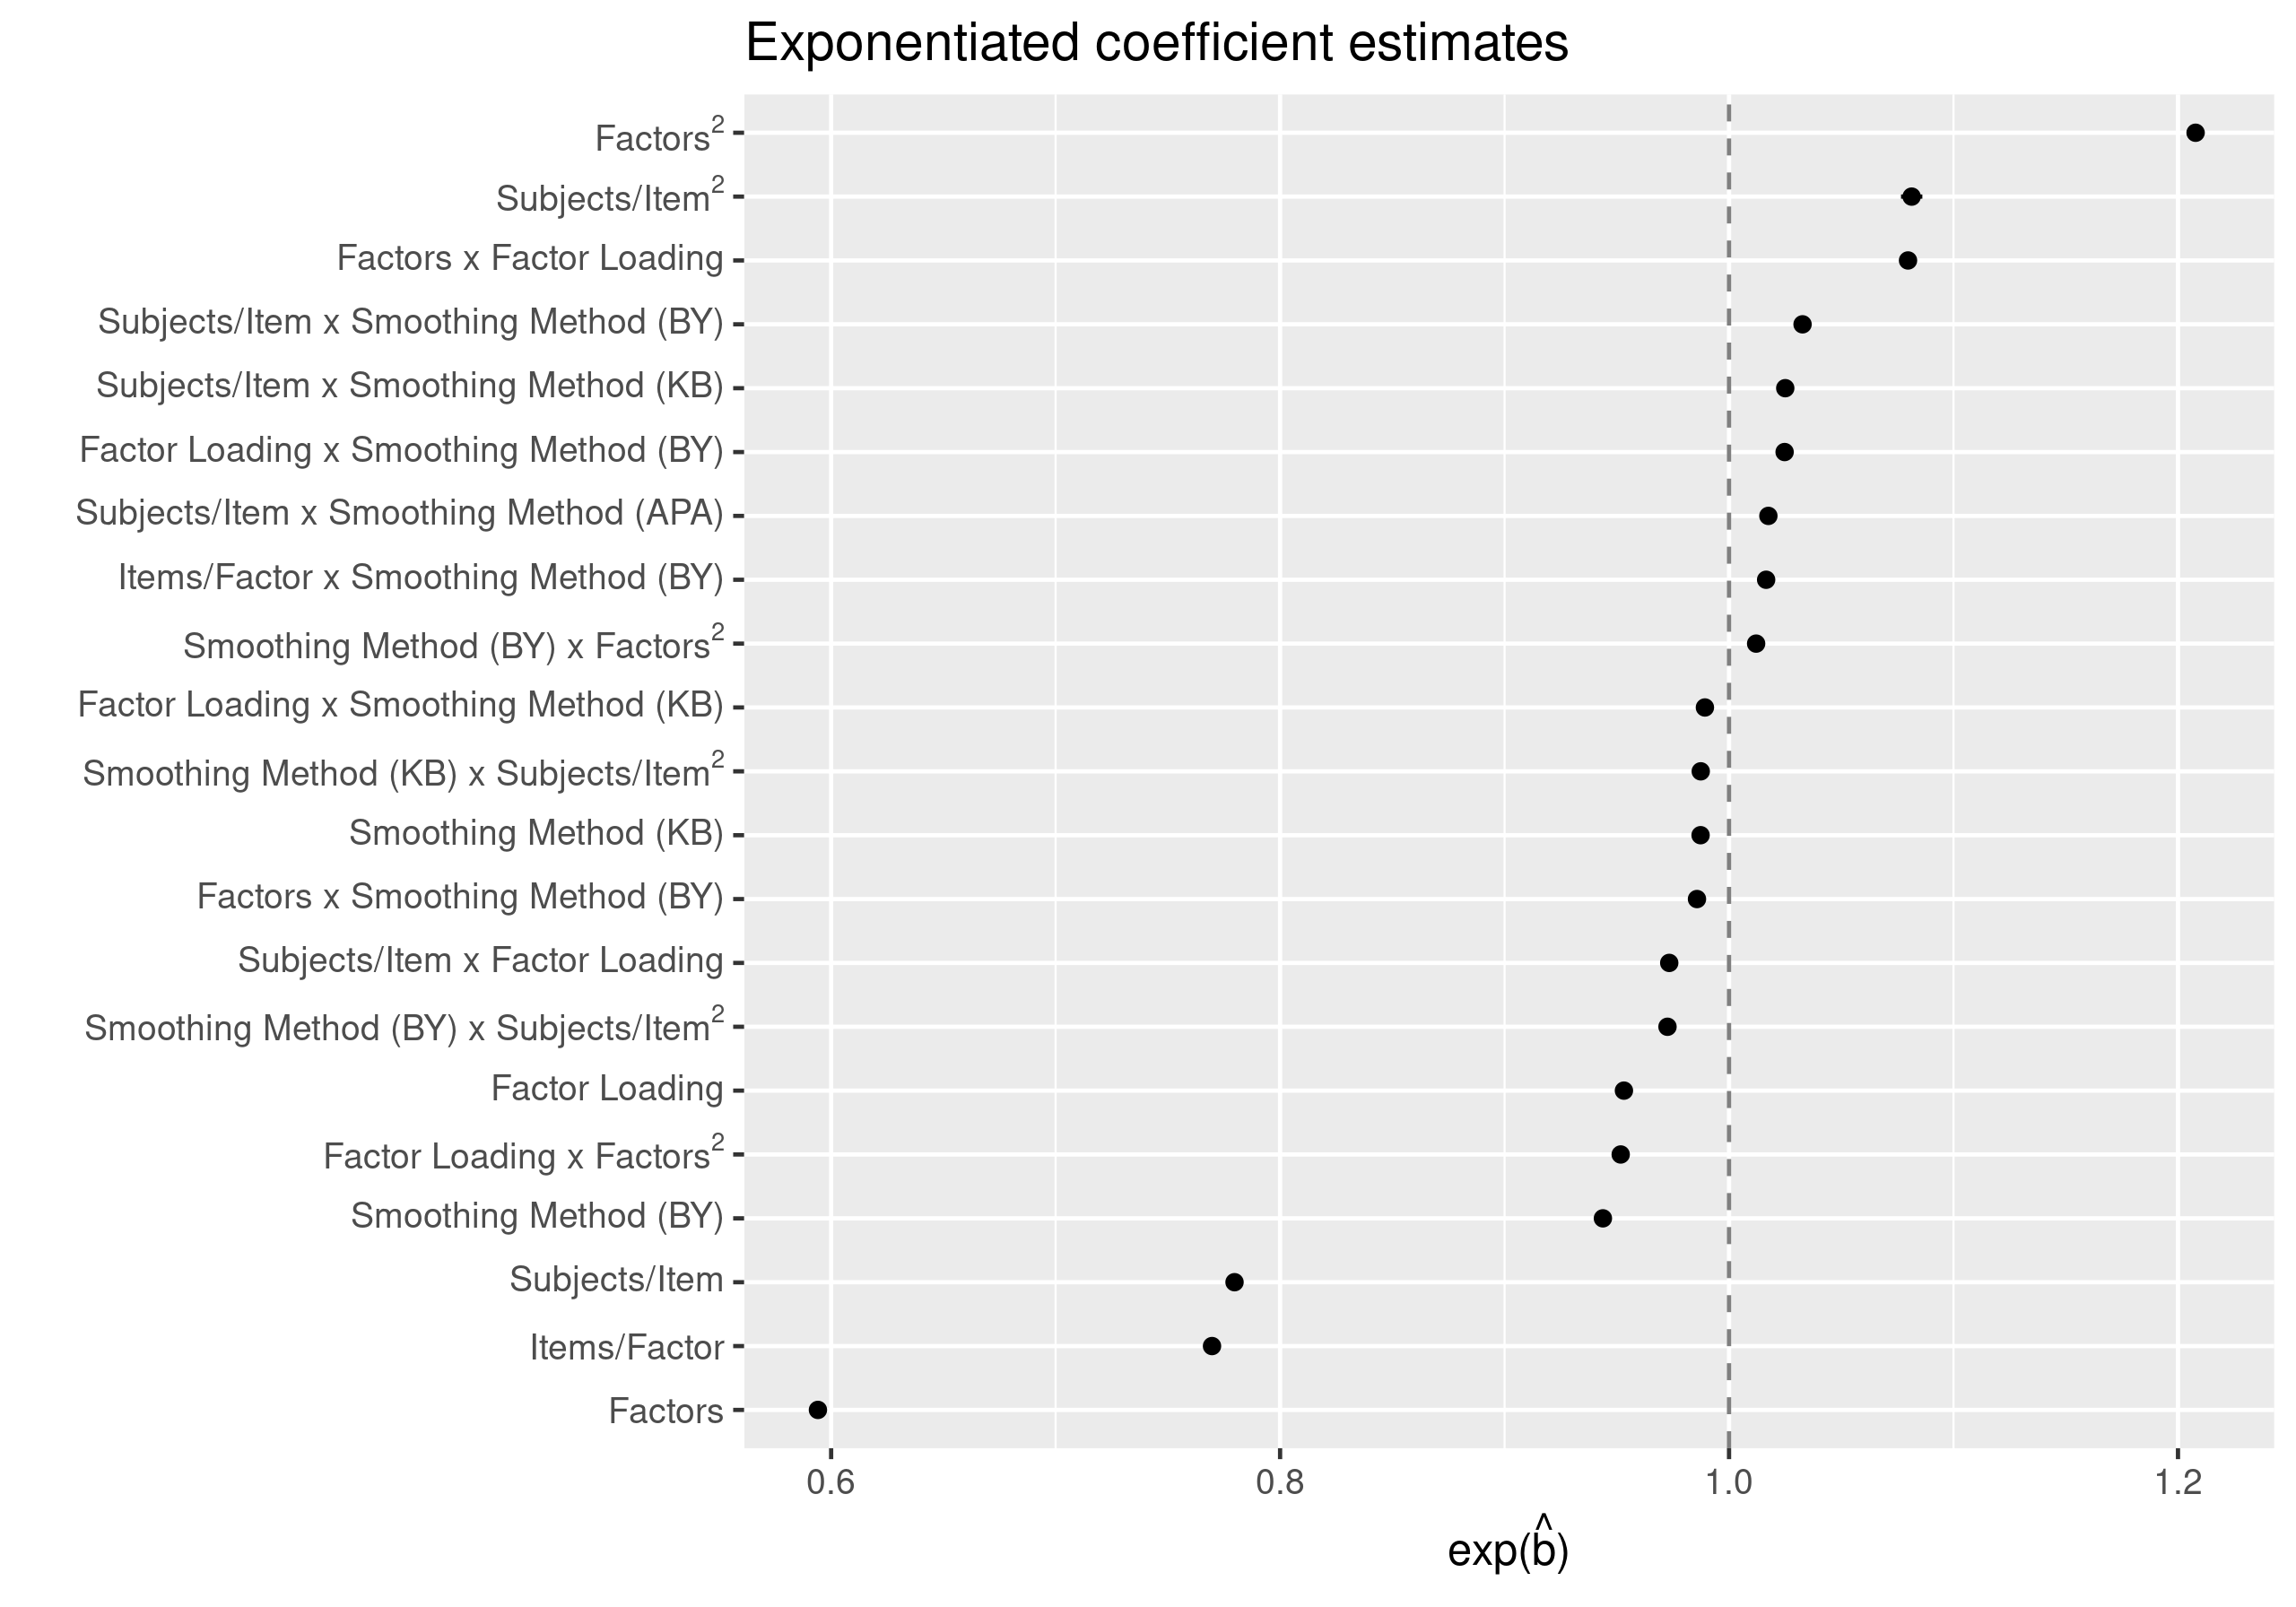
\includegraphics[width=1\linewidth]{/home/justin/Documents/masters_thesis/Text/figs/RpopRsm_coefplot} 

}

\caption{Exponentiated coefficient estimates for the mixed effects model using $\log[\mathrm{D}_{\mathrm{s}}(\mathbf{R}_{\textrm{Sm}}, \mathbf{R}_{\textrm{Pop}})]$ as the dependent variable (Model 1B). APA = Higham (2002); BY = Bentler-Yuan (2011); KB = Knol-Berger (1991). The effect of the condition where no smoothing was applied is subsumed within the Constant term.}\label{fig:coefplot-RpopRsm}
\end{figure}

\begin{figure}

{\centering \includegraphics[width=1\linewidth]{/home/justin/Documents/masters_thesis/Text/figs/RpopRsm_fitted_vals} 

}

\caption{Scaled distance between the smoothed ($\mathbf{R}_{\textrm{Sm}}$) and model-implied ($\mathbf{R}_{\textrm{Pop}}$) correlation matrices. APA = Higham (2002); BY = Bentler-Yuan (2011); KB = Knol-Berger (1991); None = no smoothing.}\label{fig:RpopRsm-fitted-vals}
\end{figure}

\begin{center}
\begin{longtable}{l D{)}{)}{11)0} D{)}{)}{11)0}}
\caption{Coefficient estimates and standard errors for the linear and polynomial mixed effects models using $\log[\mathrm{D}_{\mathrm{s}}(\mathbf{R}_{\textrm{Sm}}, \mathbf{R}_{\textrm{Pop}})]$ as the dependent variable and estimating a random intercept for each indefinite correlation matrix.}
\label{tab:distance-mod-summary}\\
\hline
 & \multicolumn{1}{c}{Linear Model} & \multicolumn{1}{c}{Polynomial Model} \\
\hline
\endfirsthead
\hline
 & \multicolumn{1}{c}{Linear Model} & \multicolumn{1}{c}{Polynomial Model} \\
\hline
\endhead
\hline
\endfoot
\hline
\endlastfoot
Constant                                          & -2.209 \; (0.001) & -2.339 \; (0.001) \\
Subjects/Item                                     & -0.300 \; (0.001) & -0.249 \; (0.001) \\
Items/Factor                                      & -0.229 \; (0.001) & -0.262 \; (0.001) \\
Factors                                           & -0.371 \; (0.001) & -0.521 \; (0.001) \\
Factor Loading                                    & -0.048 \; (0.001) & -0.048 \; (0.001) \\
Model Error                                       & -0.008 \; (0.001) & -0.010 \; (0.001) \\
Smoothing Method (APA)                            & -0.015 \; (0.000) & -0.009 \; (0.000) \\
Smoothing Method (BY)                             & -0.067 \; (0.000) & -0.058 \; (0.000) \\
Smoothing Method (KB)                             & -0.020 \; (0.000) & -0.013 \; (0.000) \\
Subjects/Item$^2$                                 &                   & 0.078 \; (0.002)  \\
Factors$^2$                                       &                   & 0.189 \; (0.001)  \\
Model Error$^2$                                   &                   & -0.004 \; (0.002) \\
Subjects/Item $\times$ Items/Factor               & -0.006 \; (0.001) & -0.005 \; (0.001) \\
Subjects/Item $\times$ Factors                    & 0.016 \; (0.001)  & 0.005 \; (0.001)  \\
Subjects/Item $\times$ Factor Loading             & 0.007 \; (0.001)  & -0.027 \; (0.001) \\
Subjects/Item $\times$ Model Error                & -0.001 \; (0.001) & -0.004 \; (0.001) \\
Subjects/Item $\times$ Smoothing Method (APA)     & 0.019 \; (0.000)  & 0.017 \; (0.000)  \\
Subjects/Item $\times$ Smoothing Method (BY)      & 0.038 \; (0.000)  & 0.032 \; (0.000)  \\
Subjects/Item $\times$ Smoothing Method (KB)      & 0.027 \; (0.000)  & 0.025 \; (0.000)  \\
Subjects/Item $\times$ Factors$^2$                &                   & -0.006 \; (0.001) \\
Subjects/Item $\times$ Model Error$^2$            &                   & -0.000 \; (0.001) \\
Items/Factor $\times$ Factors                     & -0.034 \; (0.001) & 0.009 \; (0.001)  \\
Items/Factor $\times$ Factor Loading              & -0.005 \; (0.001) & 0.001 \; (0.001)  \\
Items/Factor $\times$ Model Error                 & 0.002 \; (0.001)  & 0.001 \; (0.001)  \\
Items/Factor $\times$ Smoothing Method (APA)      & -0.000 \; (0.000) & -0.000 \; (0.000) \\
Items/Factor $\times$ Smoothing Method (BY)       & 0.018 \; (0.000)  & 0.016 \; (0.000)  \\
Items/Factor $\times$ Smoothing Method (KB)       & 0.000 \; (0.000)  & -0.000 \; (0.000) \\
Items/Factor $\times$ Subjects/Item$^2$           &                   & 0.003 \; (0.001)  \\
Items/Factor $\times$ Factors$^2$                 &                   & -0.003 \; (0.001) \\
Items/Factor $\times$ Model Error$^2$             &                   & -0.000 \; (0.001) \\
Factors $\times$ Factor Loading                   & 0.033 \; (0.001)  & 0.077 \; (0.001)  \\
Factors $\times$ Model Error                      & 0.001 \; (0.001)  & -0.002 \; (0.001) \\
Factors $\times$ Smoothing Method (APA)           & 0.002 \; (0.000)  & 0.003 \; (0.000)  \\
Factors $\times$ Smoothing Method (BY)            & -0.005 \; (0.000) & -0.014 \; (0.000) \\
Factors $\times$ Smoothing Method (KB)            & -0.000 \; (0.000) & -0.002 \; (0.000) \\
Factors $\times$ Subjects/Item$^2$                &                   & 0.002 \; (0.001)  \\
Factors $\times$ Model Error$^2$                  &                   & -0.001 \; (0.001) \\
Factor Loading $\times$ Model Error               & 0.009 \; (0.001)  & 0.008 \; (0.001)  \\
Factor Loading $\times$ Smoothing Method (APA)    & -0.008 \; (0.000) & -0.008 \; (0.000) \\
Factor Loading $\times$ Smoothing Method (BY)     & 0.024 \; (0.000)  & 0.024 \; (0.000)  \\
Factor Loading $\times$ Smoothing Method (KB)     & -0.011 \; (0.000) & -0.011 \; (0.000) \\
Factor Loading $\times$ Subjects/Item$^2$         &                   & 0.002 \; (0.001)  \\
Factor Loading $\times$ Factors$^2$               &                   & -0.049 \; (0.001) \\
Factor Loading $\times$ Model Error$^2$           &                   & 0.003 \; (0.001)  \\
Model Error $\times$ Smoothing Method (APA)       & -0.003 \; (0.000) & -0.003 \; (0.000) \\
Model Error $\times$ Smoothing Method (BY)        & 0.001 \; (0.000)  & 0.000 \; (0.000)  \\
Model Error $\times$ Smoothing Method (KB)        & -0.004 \; (0.000) & -0.004 \; (0.000) \\
Model Error $\times$ Subjects/Item$^2$            &                   & 0.001 \; (0.001)  \\
Model Error $\times$ Factors$^2$                  &                   & 0.002 \; (0.001)  \\
Smoothing Method (APA) $\times$ Subjects/Item$^2$ &                   & -0.009 \; (0.000) \\
Smoothing Method (BY) $\times$ Subjects/Item$^2$  &                   & -0.028 \; (0.000) \\
Smoothing Method (KB) $\times$ Subjects/Item$^2$  &                   & -0.013 \; (0.000) \\
Smoothing Method (APA) $\times$ Factors$^2$       &                   & -0.002 \; (0.000) \\
Smoothing Method (BY) $\times$ Factors$^2$        &                   & 0.012 \; (0.000)  \\
Smoothing Method (KB) $\times$ Factors$^2$        &                   & 0.002 \; (0.000)  \\
Smoothing Method (APA) $\times$ Model Error$^2$   &                   & -0.001 \; (0.000) \\
Smoothing Method (BY) $\times$ Model Error$^2$    &                   & 0.001 \; (0.000)  \\
Smoothing Method (KB) $\times$ Model Error$^2$    &                   & -0.001 \; (0.000) \\
Subjects/Item$^2$ $\times$ Factors$^2$            &                   & 0.000 \; (0.001)  \\
Subjects/Item$^2$ $\times$ Model Error$^2$        &                   & 0.002 \; (0.002)  \\
Factors$^2$ $\times$ Model Error$^2$              &                   & 0.001 \; (0.001)  \\
\hline
AIC                                               & -1808591.524      & -1938579.038      \\
BIC                                               & -1808191.308      & -1937878.660      \\
Log Likelihood                                    & 904331.762        & 969352.519        \\
Num. obs.                                         & 497381            & 497381            \\
Num. groups: id                                   & 124346            & 124346            \\
Var: id (Intercept)                               & 0.017             & 0.008             \\
Var: Residual                                     & 0.000             & 0.000             \\
\end{longtable}
\end{center}

\hypertarget{recovery-of-factor-loadings}{%
\subsection{Recovery of Factor Loadings}\label{recovery-of-factor-loadings}}

I next analyzed the simulation results in terms of factor loading recovery. In particular, I was interested in whether factor analysis of smoothed indefinite correlation matrices led to better factor loading estimates compared to when factor analysis was conducted on the indefinite correlation matrices directly. I was also interested in whether particular smoothing methods led to better factor loading estimates than others and whether the interactions between smoothing methods and the other variables (e.g., number of items per factor, number of subjects per item, factor analysis method, etc.) affected factor loading estimation. For the purposes of these analyses, I evaluated factor loading recovery using the root-mean-square error (RMSE) between the estimated and population factor loadings for the major factors. Given a matrix of estimated major factor loadings \(\hat{\mathbf{F}} = \{ \hat{f}_{ij} \}_{p \times m}\), and the corresponding matrix of population major factor loadings, \(\mathbf{F} = \{ f_{ij} \}_{p \times m}\),
\begin{equation}
\textrm{RMSE}(\mathbf{F}, \hat{\mathbf{F}}) = \sqrt{\sum_{i = 1}^{p} \sum_{j = 1}^{m} \frac{(f_{ij} - \hat{f}_{ij})^2}{pm}}.
\label{eq:rmse}
\end{equation}

To determine which smoothing method resulted in the best factor loading estimates, I calculated the \(\textrm{RMSE}(\mathbf{F}, \hat{\mathbf{F}})\) for each pair of estimated and population factor loading matrices corresponding to the (possibly) smoothed indefinite tetrachoric correlation matrices. Relatively small \(\textrm{RMSE}(\mathbf{F}, \hat{\mathbf{F}})\) values indicated that the estimated factor loading matrices were more similar to their corresponding population factor loading matrices, whereas larger \(\textrm{RMSE}(\mathbf{F}, \hat{\mathbf{F}})\) values indicated poorly-estimated factor loading matrices. As in the previous section, the four cases where the Higham (2002) algorithm did not converge were not included in my analyses. Furthermore, cases where PA failed to converge were also not included. In total, there were 2,714 cases where the PA algorithm did not converge (convergence rate = 99.5\%) and only four cases where the ML algorithm did not converge (convergence rate \textgreater{} 99.9\%).

Using the converged data, I fit a mixed-effects model (Model 2A) regressing \(\log \textrm{RMSE}(\mathbf{F}, \hat{\mathbf{F}})\) on number of subjects per item, number of items per factor, number of factors, factor loading, model error, smoothing algorithm, factor analysis method (PA, OLS, or ML), all two-way interactions between these variables, and a random intercept estimated for every unique indefinite correlation matrix.\footnote{All numeric predictors were scaled to have a mean of zero and variance of one prior to analysis. Diagnostic plots can be found in Appendix A.} I also fit a second mixed-effects model (Model 2B) with additional second-degree polynomial terms for number of subjects per item, number of factors, and factor loading. The results for both models are summarized in Table \ref{tab:loading-mod-summary} and indicated that Model 2B should be preferred to Model 2A based on the AIC and BIC criteria. Therefore, coefficient estimates and estimated marginal means reported in this section were obtained using Model 2B.

To show the variables that most affected \(\log \textrm{RMSE}(\mathbf{F}, \hat{\mathbf{F}})\), ordered, exponentiated coefficient estimates with 99\% confidence intervals for Model 2B are shown in Figure \ref{fig:coefplot-loading-recovery} (note that exponentiated coefficients less than 1.01 and greater than 0.99 were omitted to conserve space). Figure \ref{fig:coefplot-loading-recovery} shows that factor loading, items per factor, number of factors, model error, and subjects per item had relatively large effects on \(\log \textrm{RMSE}(\mathbf{F}, \hat{\mathbf{F}})\). Additionally, many of the polynomial terms and interactions between these variables also had relatively large estimated effects (see Figure \ref{fig:coefplot-loading-recovery} and Table \ref{tab:loading-mod-summary}). To better understand the effects of each of these design variables on \(\textrm{RMSE}(\mathbf{F}, \hat{\mathbf{F}})\), Figure \ref{fig:loading-mm} shows estimated marginal means conditioned on number of factors, model error, number of subjects per item, number of items per factor, smoothing method, factor extraction method, and factor loading. As in the previous section, estimated marginal means were used instead of raw means because each condition of the design had a different number of observations due to only using results for indefinite tetrachoric correlation matrices.

Concerning the primary question of interest in this section, the coefficient estimates from Model 2B (and the marginal means shown in Figure \ref{fig:loading-mm}) indicated that choice of smoothing method generally had little impact on \(\textrm{RMSE}(\mathbf{F}, \hat{\mathbf{F}})\). Of the effects involving smoothing methods, only the effects involving the Bentler-Yuan algorithm were non-negligible. Therefore, only the application of the Bentler-Yuan algorithm to indefinite tetrachoric correlation matrices seemed to be related to any improvement (or indeed, difference) in \(\textrm{RMSE}(\mathbf{F}, \hat{\mathbf{F}})\) values when used for factor analysis. Moreover, even the estimated main effect associated with the Bentler-Yuan algorithm (2011) was quite modest (\(\hat{b} = -0.03\), \(SE = 0.00\), \(e^{-0.03} = 0.97\)) and was offset by the positive estimated interaction effects with factor loading (\(\hat{b} = 0.02\), \(SE = 0.00\), \(e^{0.02} = 1.02\)) and items per factor (\(\hat{b} = 0.02\), \(SE = 0.00\), \(e^{0.02} = 1.02\)). These effects are evident in Figure \ref{fig:loading-mm}, which shows that the Bentler-Yuan algorithm (2011) led to slightly lower \(\textrm{RMSE}(\mathbf{F}, \hat{\mathbf{F}})\) values for conditions with low factor loadings and few items per factor, but led to nearly identical results to the alternative methods as factor loading magnitude and number of items per factor increased.

Although choice of smoothing method did not have a large influence on factor loading recovery, the other design variables did have an influence on \(\textrm{RMSE}(\mathbf{F}, \hat{\mathbf{F}})\) values. The effects of these other variables (including interactions and polynomial terms) are best understood using the marginal means shown in Figure \ref{fig:loading-mm}. Considering first the effect of factor loading, Figure \ref{fig:loading-mm} shows that \(\textrm{RMSE}(\mathbf{F}, \hat{\mathbf{F}})\) values tended to decrease as factor loadings increased (\(\hat{b} = -0.57\), \(SE = 0.00\), \(e^{-0.57} = 0.57\)). Interestingly, there was also a relatively large interaction between factor loading and ML factor extraction (\(\hat{b} = 0.22\), \(SE = 0.00\), \(e^{0.22} = 1.25\)) such that ML seemed to benefit less than PA or OLS from higher factor loadings.

After factor loading, the number of items per factor had the largest estimated effect on \(\textrm{RMSE}(\mathbf{F}, \hat{\mathbf{F}})\) values (\(\hat{b} = -0.37\), \(SE = 0.00\), \(e^{-0.37} = 0.69\)). As can be seen in Figure \ref{fig:loading-mm}, increasing the number of items per factor tended to improve factor loading recovery (i.e., led to lower \(\textrm{RMSE}(\mathbf{F}, \hat{\mathbf{F}})\) values). There was a similar (albeit smaller) effect for the number of subjects per item, such that increasing the number of subjects per item tended to lead to smaller \(\textrm{RMSE}(\mathbf{F}, \hat{\mathbf{F}})\) values (\(\hat{b} = -0.18\), \(SE = 0.00\), \(e^{-0.18} = 0.84\)). However, both the effects of number of items per factor and number of subjects per item were affected by their associated polynomial terms and interactions. For instance, the effect of increasing the number of items per factor was largest when factor loadings were relatively small, as indicated by the interaction between the number of items per factor and squared factor loadings (\(\hat{b} = 0.14\), \(SE = 0.00\), \(e^{0.14} = 1.15\)). The effect of the number of items per factor was also influenced by model error (as will be discussed shortly). Concerning the effect of the number of subjects per item, there was a large estimated effect for squared number of subjects per item such that the beneficial effect of increasing the number of subjects dissipated as the number of subjects per item increased (\(\hat{b} = 0.16\), \(SE = 0.00\), \(e^{0.16} = 1.17\)).

Concerning the effect of number of factors on \(\textrm{RMSE}(\mathbf{F}, \hat{\mathbf{F}})\) values, Figure \ref{fig:loading-mm} shows that \(\textrm{RMSE}(\mathbf{F}, \hat{\mathbf{F}})\) values tended to be lower for conditions with more factors compared to those with fewer factors (\(\hat{b} = -0.34\), \(SE = 0.00\), \(e^{-0.34} = 0.71\)). Moreover, the decrease in \(\textrm{RMSE}(\mathbf{F}, \hat{\mathbf{F}})\) seemed to be nonlinear, such that the effect of increasing the number of factors was largest when there were relatively few factors, as indicated by the quadratic term for number of factors (\(\hat{b} = 0.09\), \(SE = 0.00\), \(e^{0.09} = 1.09\)). On its face, these effects seem to suggest that models with large numbers of major factors led to better factor loading recovery than those with fewer factors. However, another explanation for this effect involves the total numbers of subjects and items. Whereas number of items per factor and number of subjects per item were fully-crossed with number of factors, the total sample size and total number of items for each data set were confounded with number of factors. In other words, conditions with larger numbers of factors tended to include more total subjects and items. The strong relationship between \(\log \textrm{RMSE}(\mathbf{F}, \hat{\mathbf{F}})\) and sample size can be clearly seen in Figure \ref{fig:RMSE-sample-size}, which shows that \(\log \textrm{RMSE}(\mathbf{F}, \hat{\mathbf{F}})\) decreased as sample size increased. Therefore, it seems reasonable that the effect of number of factors might be better understood as being related to the total number of items and subjects in a data set. Similarly, the negative interaction between number of factors and ML (\(\hat{b} = -0.20\), \(SE = 0.00\), \(e^{-0.20} = 0.82\)) could be interpreted instead as an interaction between total number of items or subjects and ML.

Moving next to model error, Model 2B indicated that increasing the proportion of uniqueness variance accounted for by the minor factors (\(\upsilon_\textrm{E}\)) was associated with worse factor loading recovery (\(\hat{b} = 0.16\), \(SE = 0.00\), \(e^{0.16} = 1.17\)). Additionally, the detrimental effect of model error on factor loading recovery seemed to worsen as the number of factors and number of items per factor increased (see Figure \ref{fig:loading-mm} and Table \ref{tab:loading-mod-summary}). On the other hand, model error seemed to have less of an impact on \(\textrm{RMSE}(\mathbf{F}, \hat{\mathbf{F}})\) as factor loadings increased, as can also be seen in Figure \ref{fig:loading-mm}. A potential explanation for this effect is that model error accounted for less of the total variance in conditions with high factor loadings because the levels of model error were defined as proportions of the uniqueness variance. I.e., conditions with high factor loadings had small uniqueness variances and correspondingly small model error variances.

Another notable effect involving model approximation error was the interaction between model error and ML factor extraction (\(\hat{b} = -0.03\), \(SE = 0.00\), \(e^{-0.03} = 0.97\)). This result indicated that, of the three factor extraction methods, ML was less affected by model error than OLS or PA. Moreover, the main effect of ML indicated that it led to lower overall \(\textrm{RMSE}(\mathbf{F}, \hat{\mathbf{F}})\) values than OLS or PA when all other variables were held constant (\(\hat{b} = -0.05\), \(SE = 0.00\), \(e^{-0.05} = 0.95\)). However, the previously-discussed interactions between ML and factor loading, number of items per factor, and number of subjects per item indicated that ML led to better results than PA or OLS only when the numbers of subjects per item and items per factor were small and factor loadings were low. In conditions with higher numbers of subjects and items, OLS and PA led to better (and highly similar) results in terms of \(\textrm{RMSE}(\mathbf{F}, \hat{\mathbf{F}})\) values.

\begin{figure}

{\centering 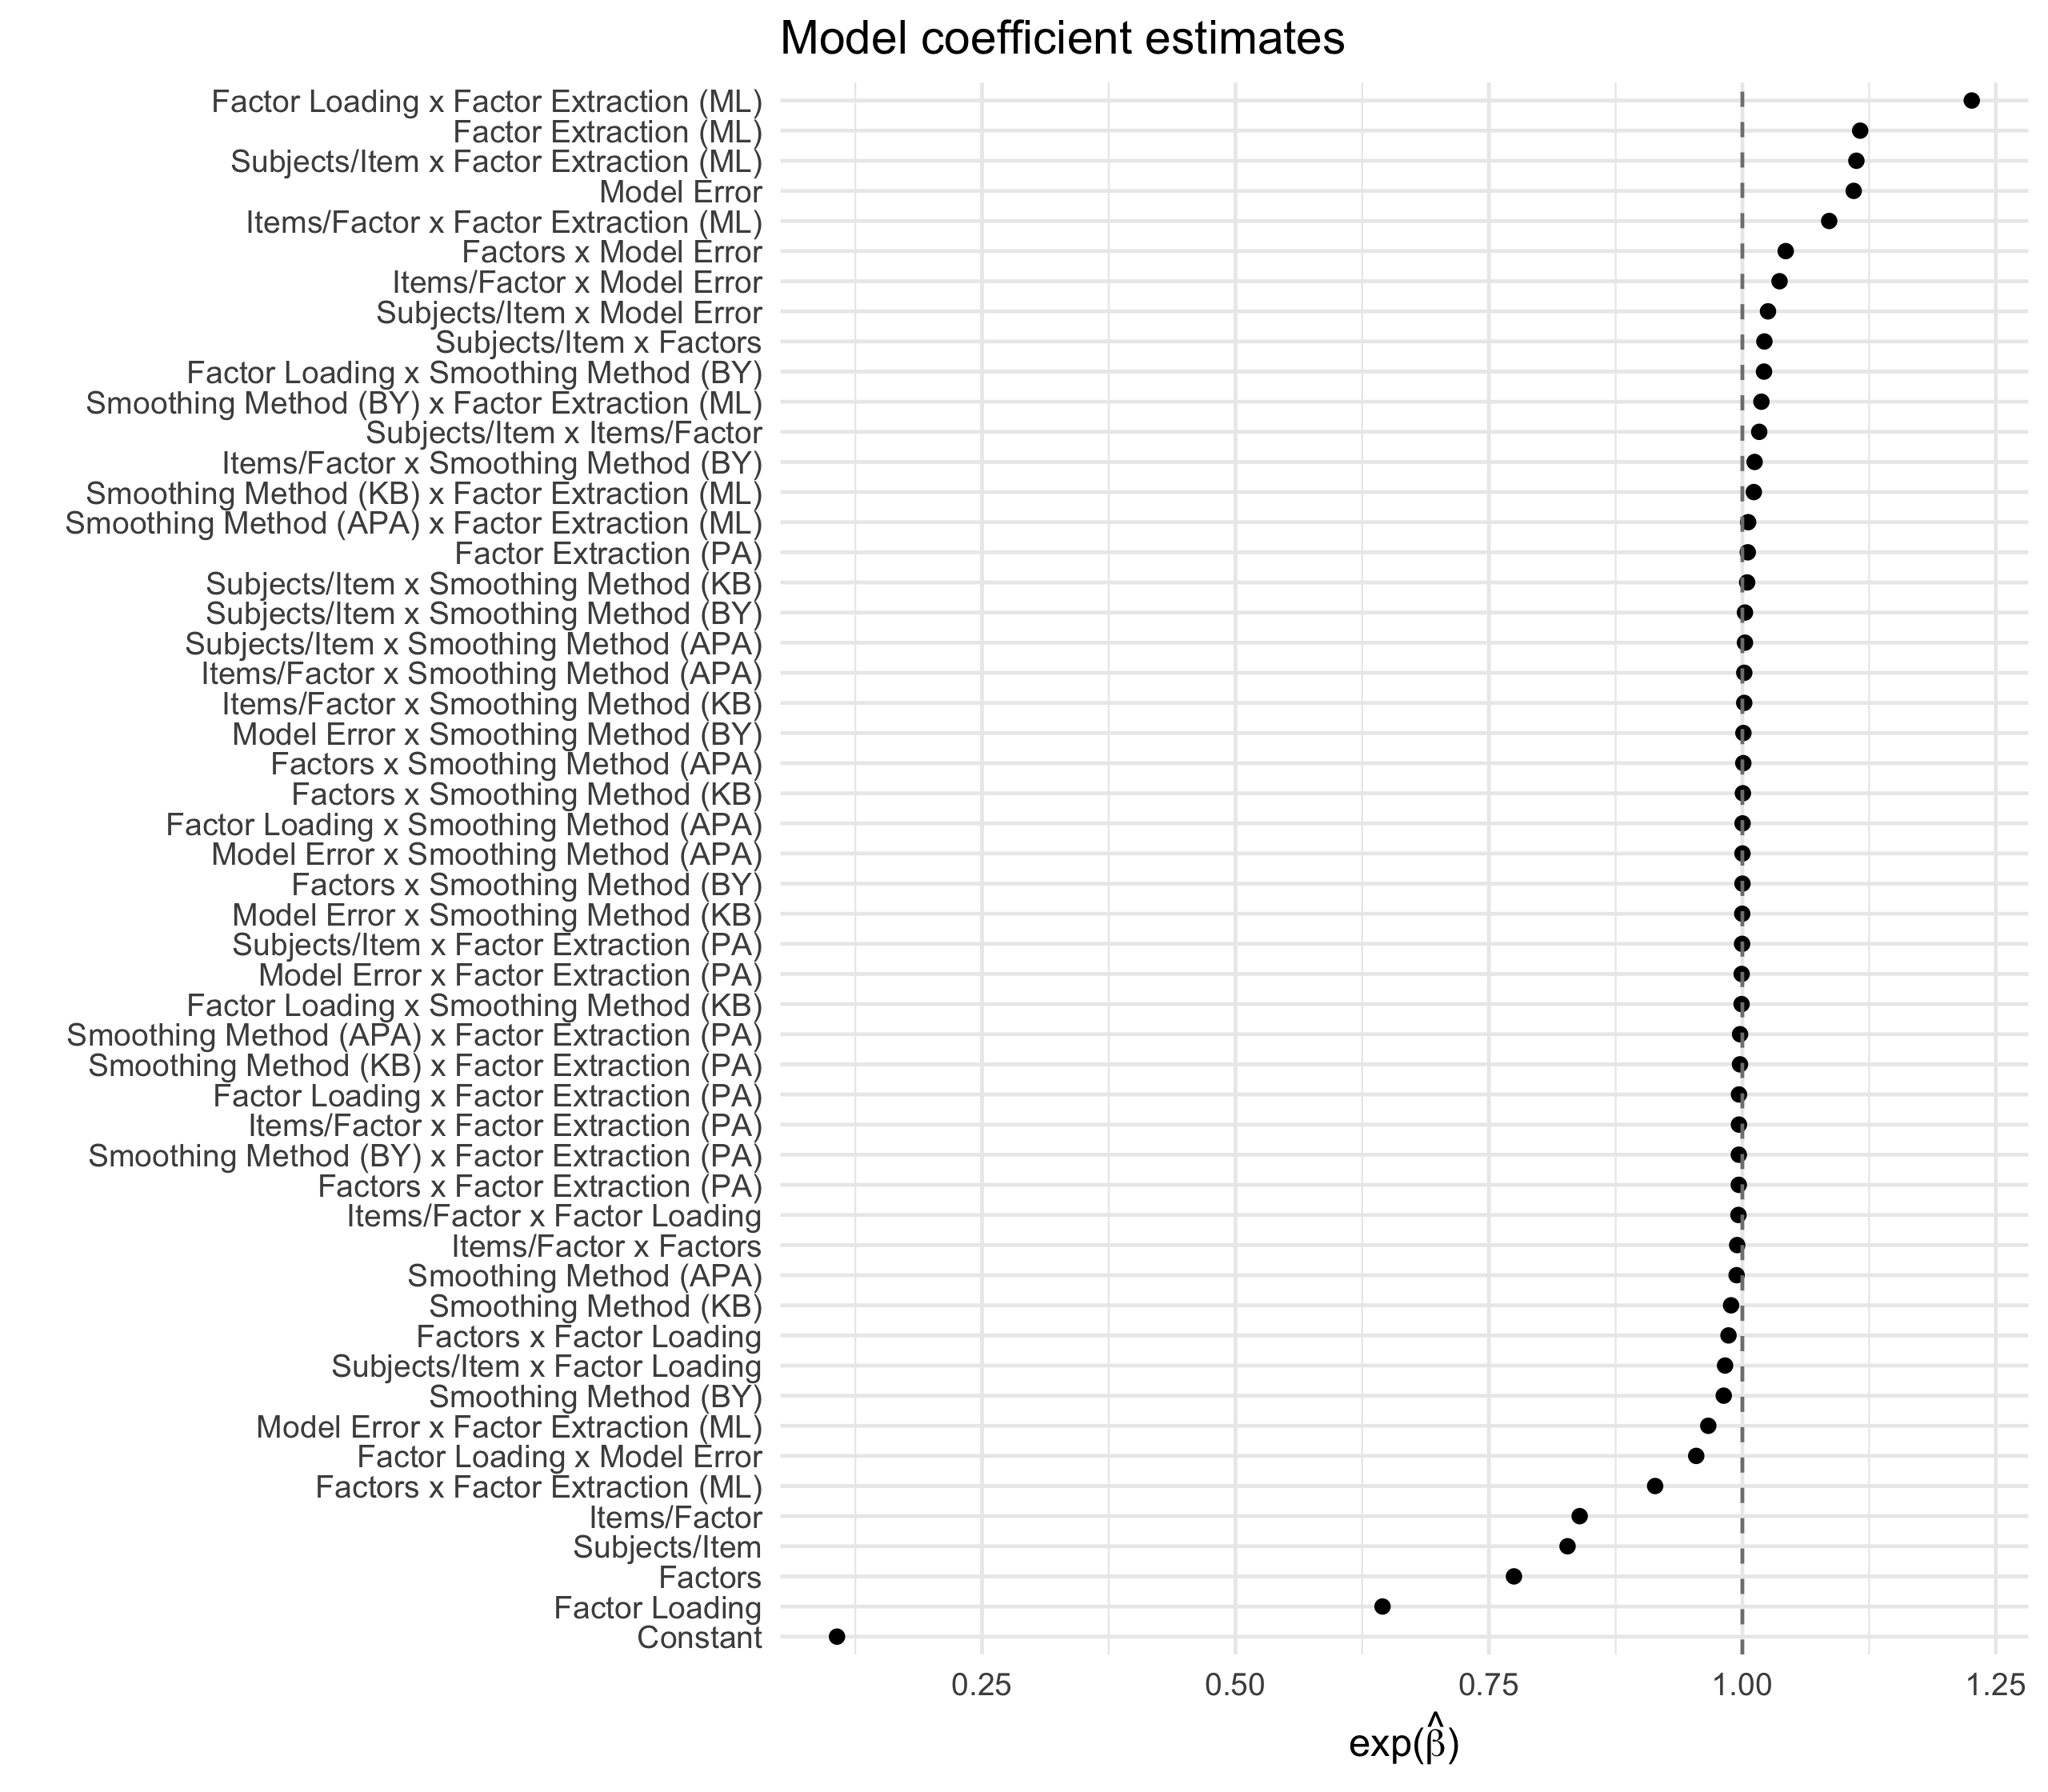
\includegraphics[width=1\linewidth]{/home/justin/Documents/masters_thesis/Text/figs/loadings_coefplot} 

}

\caption{Exponentiated coefficient estimates for the mixed effects model using $\log[\textrm{RMSE}(\mathbf{F}, \hat{\mathbf{F}})]$ as the dependent variable (Model 2B). APA = Higham (2002); BY = Bentler-Yuan (2011); KB = Knol-Berger (1991); ML = Maximum likelihood; PA = Principal axis. The effects of no smoothing and ordinary least squares factor analysis are subsumed within the Constant term.}\label{fig:coefplot-loading-recovery}
\end{figure}

\begin{center}
\begin{longtable}{l D{)}{)}{11)0} D{)}{)}{11)0}}
\caption{Coefficient estimates and standard errors for the linear and polynomial mixed effects models using $\log[\textrm{RMSE}(\mathbf{F}, \hat{\mathbf{F}})]$ as the dependent variable and estimating a random intercept for each indefinite correlation matrix.}
\label{tab:loading-mod-summary}\\
\hline
 & \multicolumn{1}{c}{Linear Model} & \multicolumn{1}{c}{Polynomial Model} \\
\hline
\endfirsthead
\hline
 & \multicolumn{1}{c}{Linear Model} & \multicolumn{1}{c}{Polynomial Model} \\
\hline
\endhead
\hline
\endfoot
\hline
\endlastfoot
Constant                                               & -2.235 \; (0.001) & -2.229 \; (0.003) \\
Subjects/Item                                          & -0.189 \; (0.001) & -0.183 \; (0.003) \\
Items/Factor                                           & -0.175 \; (0.001) & -0.369 \; (0.002) \\
Factors                                                & -0.255 \; (0.001) & -0.344 \; (0.002) \\
Factor Loading                                         & -0.438 \; (0.001) & -0.574 \; (0.002) \\
Model Error                                            & 0.104 \; (0.001)  & 0.229 \; (0.002)  \\
Smoothing Method (APA)                                 & -0.006 \; (0.000) & -0.004 \; (0.001) \\
Smoothing Method (BY)                                  & -0.019 \; (0.000) & -0.033 \; (0.001) \\
Smoothing Method (KB)                                  & -0.011 \; (0.000) & -0.008 \; (0.001) \\
Extraction Method (ML)                                 & 0.110 \; (0.000)  & -0.049 \; (0.001) \\
Extraction Method (PA)                                 & 0.005 \; (0.000)  & 0.004 \; (0.001)  \\
Subjects/Item$^2$                                      &                   & 0.157 \; (0.003)  \\
Factor Loading$^2$                                     &                   & 0.006 \; (0.003)  \\
Factors$^2$                                            &                   & 0.095 \; (0.002)  \\
Model Error$^2$                                        &                   & 0.099 \; (0.003)  \\
Subjects/Item $\times$ Items/Factor                    & 0.016 \; (0.001)  & 0.024 \; (0.001)  \\
Subjects/Item $\times$ Factors                         & 0.021 \; (0.001)  & 0.033 \; (0.001)  \\
Subjects/Item $\times$ Factor Loading                  & -0.017 \; (0.001) & -0.076 \; (0.003) \\
Subjects/Item $\times$ Model Error                     & 0.025 \; (0.001)  & 0.019 \; (0.001)  \\
Subjects/Item $\times$ Smoothing Method (APA)          & 0.003 \; (0.000)  & 0.003 \; (0.000)  \\
Subjects/Item $\times$ Smoothing Method (BY)           & 0.003 \; (0.000)  & 0.001 \; (0.000)  \\
Subjects/Item $\times$ Smoothing Method (KB)           & 0.005 \; (0.000)  & 0.006 \; (0.000)  \\
Subjects/Item $\times$ Extraction Method (ML)          & 0.107 \; (0.000)  & 0.146 \; (0.000)  \\
Subjects/Item $\times$ Extraction Method (PA)          & -0.000 \; (0.000) & -0.000 \; (0.000) \\
Subjects/Item $\times$ Factor Loading$^2$              &                   & -0.004 \; (0.004) \\
Subjects/Item $\times$ Factors$^2$                     &                   & -0.020 \; (0.001) \\
Subjects/Item $\times$ Model Error$^2$                 &                   & 0.012 \; (0.002)  \\
Items/Factor $\times$ Factors                          & -0.005 \; (0.001) & 0.041 \; (0.001)  \\
Items/Factor $\times$ Factor Loading                   & -0.004 \; (0.001) & -0.052 \; (0.001) \\
Items/Factor $\times$ Model Error                      & 0.036 \; (0.001)  & 0.054 \; (0.001)  \\
Items/Factor $\times$ Smoothing Method (APA)           & 0.002 \; (0.000)  & 0.003 \; (0.000)  \\
Items/Factor $\times$ Smoothing Method (BY)            & 0.012 \; (0.000)  & 0.017 \; (0.000)  \\
Items/Factor $\times$ Smoothing Method (KB)            & 0.002 \; (0.000)  & 0.002 \; (0.000)  \\
Items/Factor $\times$ Extraction Method (ML)           & 0.082 \; (0.000)  & 0.102 \; (0.000)  \\
Items/Factor $\times$ Extraction Method (PA)           & -0.003 \; (0.000) & -0.005 \; (0.000) \\
Items/Factor $\times$ Subjects/Item$^2$                &                   & -0.005 \; (0.001) \\
Items/Factor $\times$ Factor Loading$^2$               &                   & 0.144 \; (0.001)  \\
Items/Factor $\times$ Factors$^2$                      &                   & -0.012 \; (0.001) \\
Items/Factor $\times$ Model Error$^2$                  &                   & 0.021 \; (0.001)  \\
Factors $\times$ Factor Loading                        & -0.014 \; (0.001) & -0.014 \; (0.001) \\
Factors $\times$ Model Error                           & 0.042 \; (0.001)  & 0.068 \; (0.001)  \\
Factors $\times$ Smoothing Method (APA)                & 0.001 \; (0.000)  & 0.001 \; (0.000)  \\
Factors $\times$ Smoothing Method (BY)                 & 0.000 \; (0.000)  & -0.003 \; (0.000) \\
Factors $\times$ Smoothing Method (KB)                 & 0.001 \; (0.000)  & -0.000 \; (0.000) \\
Factors $\times$ Extraction Method (ML)                & -0.090 \; (0.000) & -0.203 \; (0.000) \\
Factors $\times$ Extraction Method (PA)                & -0.004 \; (0.000) & -0.006 \; (0.000) \\
Factors $\times$ Subjects/Item$^2$                     &                   & -0.007 \; (0.002) \\
Factors $\times$ Factor Loading$^2$                    &                   & -0.073 \; (0.002) \\
Factors $\times$ Model Error$^2$                       &                   & 0.026 \; (0.002)  \\
Factor Loading $\times$ Model Error                    & -0.047 \; (0.001) & -0.023 \; (0.001) \\
Factor Loading $\times$ Smoothing Method (APA)         & 0.000 \; (0.000)  & 0.000 \; (0.000)  \\
Factor Loading $\times$ Smoothing Method (BY)          & 0.021 \; (0.000)  & 0.022 \; (0.000)  \\
Factor Loading $\times$ Smoothing Method (KB)          & -0.001 \; (0.000) & -0.001 \; (0.000) \\
Factor Loading $\times$ Extraction Method (ML)         & 0.204 \; (0.000)  & 0.217 \; (0.000)  \\
Factor Loading $\times$ Extraction Method (PA)         & -0.003 \; (0.000) & -0.004 \; (0.000) \\
Factor Loading $\times$ Subjects/Item$^2$              &                   & 0.004 \; (0.003)  \\
Factor Loading $\times$ Factors$^2$                    &                   & 0.018 \; (0.001)  \\
Factor Loading $\times$ Model Error$^2$                &                   & 0.003 \; (0.002)  \\
Model Error $\times$ Smoothing Method (APA)            & 0.000 \; (0.000)  & 0.000 \; (0.000)  \\
Model Error $\times$ Smoothing Method (BY)             & 0.001 \; (0.000)  & 0.001 \; (0.000)  \\
Model Error $\times$ Smoothing Method (KB)             & -0.000 \; (0.000) & -0.000 \; (0.000) \\
Model Error $\times$ Extraction Method (ML)            & -0.034 \; (0.000) & -0.035 \; (0.000) \\
Model Error $\times$ Extraction Method (PA)            & -0.001 \; (0.000) & -0.001 \; (0.000) \\
Model Error $\times$ Subjects/Item$^2$                 &                   & -0.034 \; (0.001) \\
Model Error $\times$ Factor Loading$^2$                &                   & -0.117 \; (0.001) \\
Model Error $\times$ Factors$^2$                       &                   & -0.022 \; (0.001) \\
Smoothing Method (APA) $\times$ Extraction Method (ML) & 0.006 \; (0.001)  & 0.006 \; (0.000)  \\
Smoothing Method (BY) $\times$ Extraction Method (ML)  & 0.019 \; (0.001)  & 0.019 \; (0.000)  \\
Smoothing Method (KB) $\times$ Extraction Method (ML)  & 0.011 \; (0.001)  & 0.011 \; (0.000)  \\
Smoothing Method (APA) $\times$ Extraction Method (PA) & -0.002 \; (0.001) & -0.002 \; (0.000) \\
Smoothing Method (BY) $\times$ Extraction Method (PA)  & -0.004 \; (0.001) & -0.003 \; (0.000) \\
Smoothing Method (KB) $\times$ Extraction Method (PA)  & -0.002 \; (0.001) & -0.002 \; (0.000) \\
Smoothing Method (APA) $\times$ Subjects/Item$^2$      &                   & -0.002 \; (0.000) \\
Smoothing Method (BY) $\times$ Subjects/Item$^2$       &                   & -0.011 \; (0.000) \\
Smoothing Method (KB) $\times$ Subjects/Item$^2$       &                   & -0.004 \; (0.000) \\
Smoothing Method (APA) $\times$ Factor Loading$^2$     &                   & 0.001 \; (0.000)  \\
Smoothing Method (BY) $\times$ Factor Loading$^2$      &                   & 0.016 \; (0.000)  \\
Smoothing Method (KB) $\times$ Factor Loading$^2$      &                   & 0.001 \; (0.000)  \\
Smoothing Method (APA) $\times$ Factors$^2$            &                   & 0.000 \; (0.000)  \\
Smoothing Method (BY) $\times$ Factors$^2$             &                   & 0.005 \; (0.000)  \\
Smoothing Method (KB) $\times$ Factors$^2$             &                   & 0.001 \; (0.000)  \\
Smoothing Method (APA) $\times$ Model Error$^2$        &                   & -0.000 \; (0.000) \\
Smoothing Method (BY) $\times$ Model Error$^2$         &                   & -0.001 \; (0.000) \\
Smoothing Method (KB) $\times$ Model Error$^2$         &                   & -0.000 \; (0.000) \\
Extraction Method (ML) $\times$ Subjects/Item$^2$      &                   & 0.011 \; (0.000)  \\
Extraction Method (PA) $\times$ Subjects/Item$^2$      &                   & 0.001 \; (0.000)  \\
Extraction Method (ML) $\times$ Factor Loading$^2$     &                   & 0.105 \; (0.000)  \\
Extraction Method (PA) $\times$ Factor Loading$^2$     &                   & 0.001 \; (0.000)  \\
Extraction Method (ML) $\times$ Factors$^2$            &                   & 0.139 \; (0.000)  \\
Extraction Method (PA) $\times$ Factors$^2$            &                   & 0.004 \; (0.000)  \\
Extraction Method (ML) $\times$ Model Error$^2$        &                   & -0.016 \; (0.000) \\
Extraction Method (PA) $\times$ Model Error$^2$        &                   & -0.000 \; (0.000) \\
Subjects/Item$^2$ $\times$ Factor Loading$^2$          &                   & -0.087 \; (0.004) \\
Subjects/Item$^2$ $\times$ Factors$^2$                 &                   & 0.010 \; (0.002)  \\
Subjects/Item$^2$ $\times$ Model Error$^2$             &                   & -0.003 \; (0.002) \\
Factor Loading$^2$ $\times$ Factors$^2$                &                   & 0.040 \; (0.002)  \\
Factor Loading$^2$ $\times$ Model Error$^2$            &                   & -0.052 \; (0.002) \\
Factors$^2$ $\times$ Model Error$^2$                   &                   & -0.027 \; (0.002) \\
\hline
AIC                                                    & -2414463.669      & -2801683.227      \\
BIC                                                    & -2413804.118      & -2800461.837      \\
Log Likelihood                                         & 1207285.834       & 1400941.614       \\
Num. obs.                                              & 1489425           & 1489425           \\
Num. groups: id                                        & 124346            & 124346            \\
Var: id (Intercept)                                    & 0.032             & 0.017             \\
Var: Residual                                          & 0.008             & 0.007             \\
\end{longtable}
\end{center}

\begin{figure}

{\centering \includegraphics[width=1\linewidth]{/home/justin/Documents/masters_thesis/Text/figs/loading_fitted_vals} 

}

\caption{Estimated marginal mean $\textrm{RMSE}(\mathbf{F}, \hat{\mathbf{F}})$ values and 99\% confidence intervals. To conserve space, the intermediate values of model error and subjects per item have been omitted. The principal axis factor extraction method was also omitted because it led to nearly identical results compared to ordinary least squares. OLS = ordinary least squares; ML = maximum likelihood; APA = Higham (2002); BY = Bentler-Yuan (2011); KB = Knol-Berger (1991).}\label{fig:loading-mm}
\end{figure}

\begin{figure}

{\centering 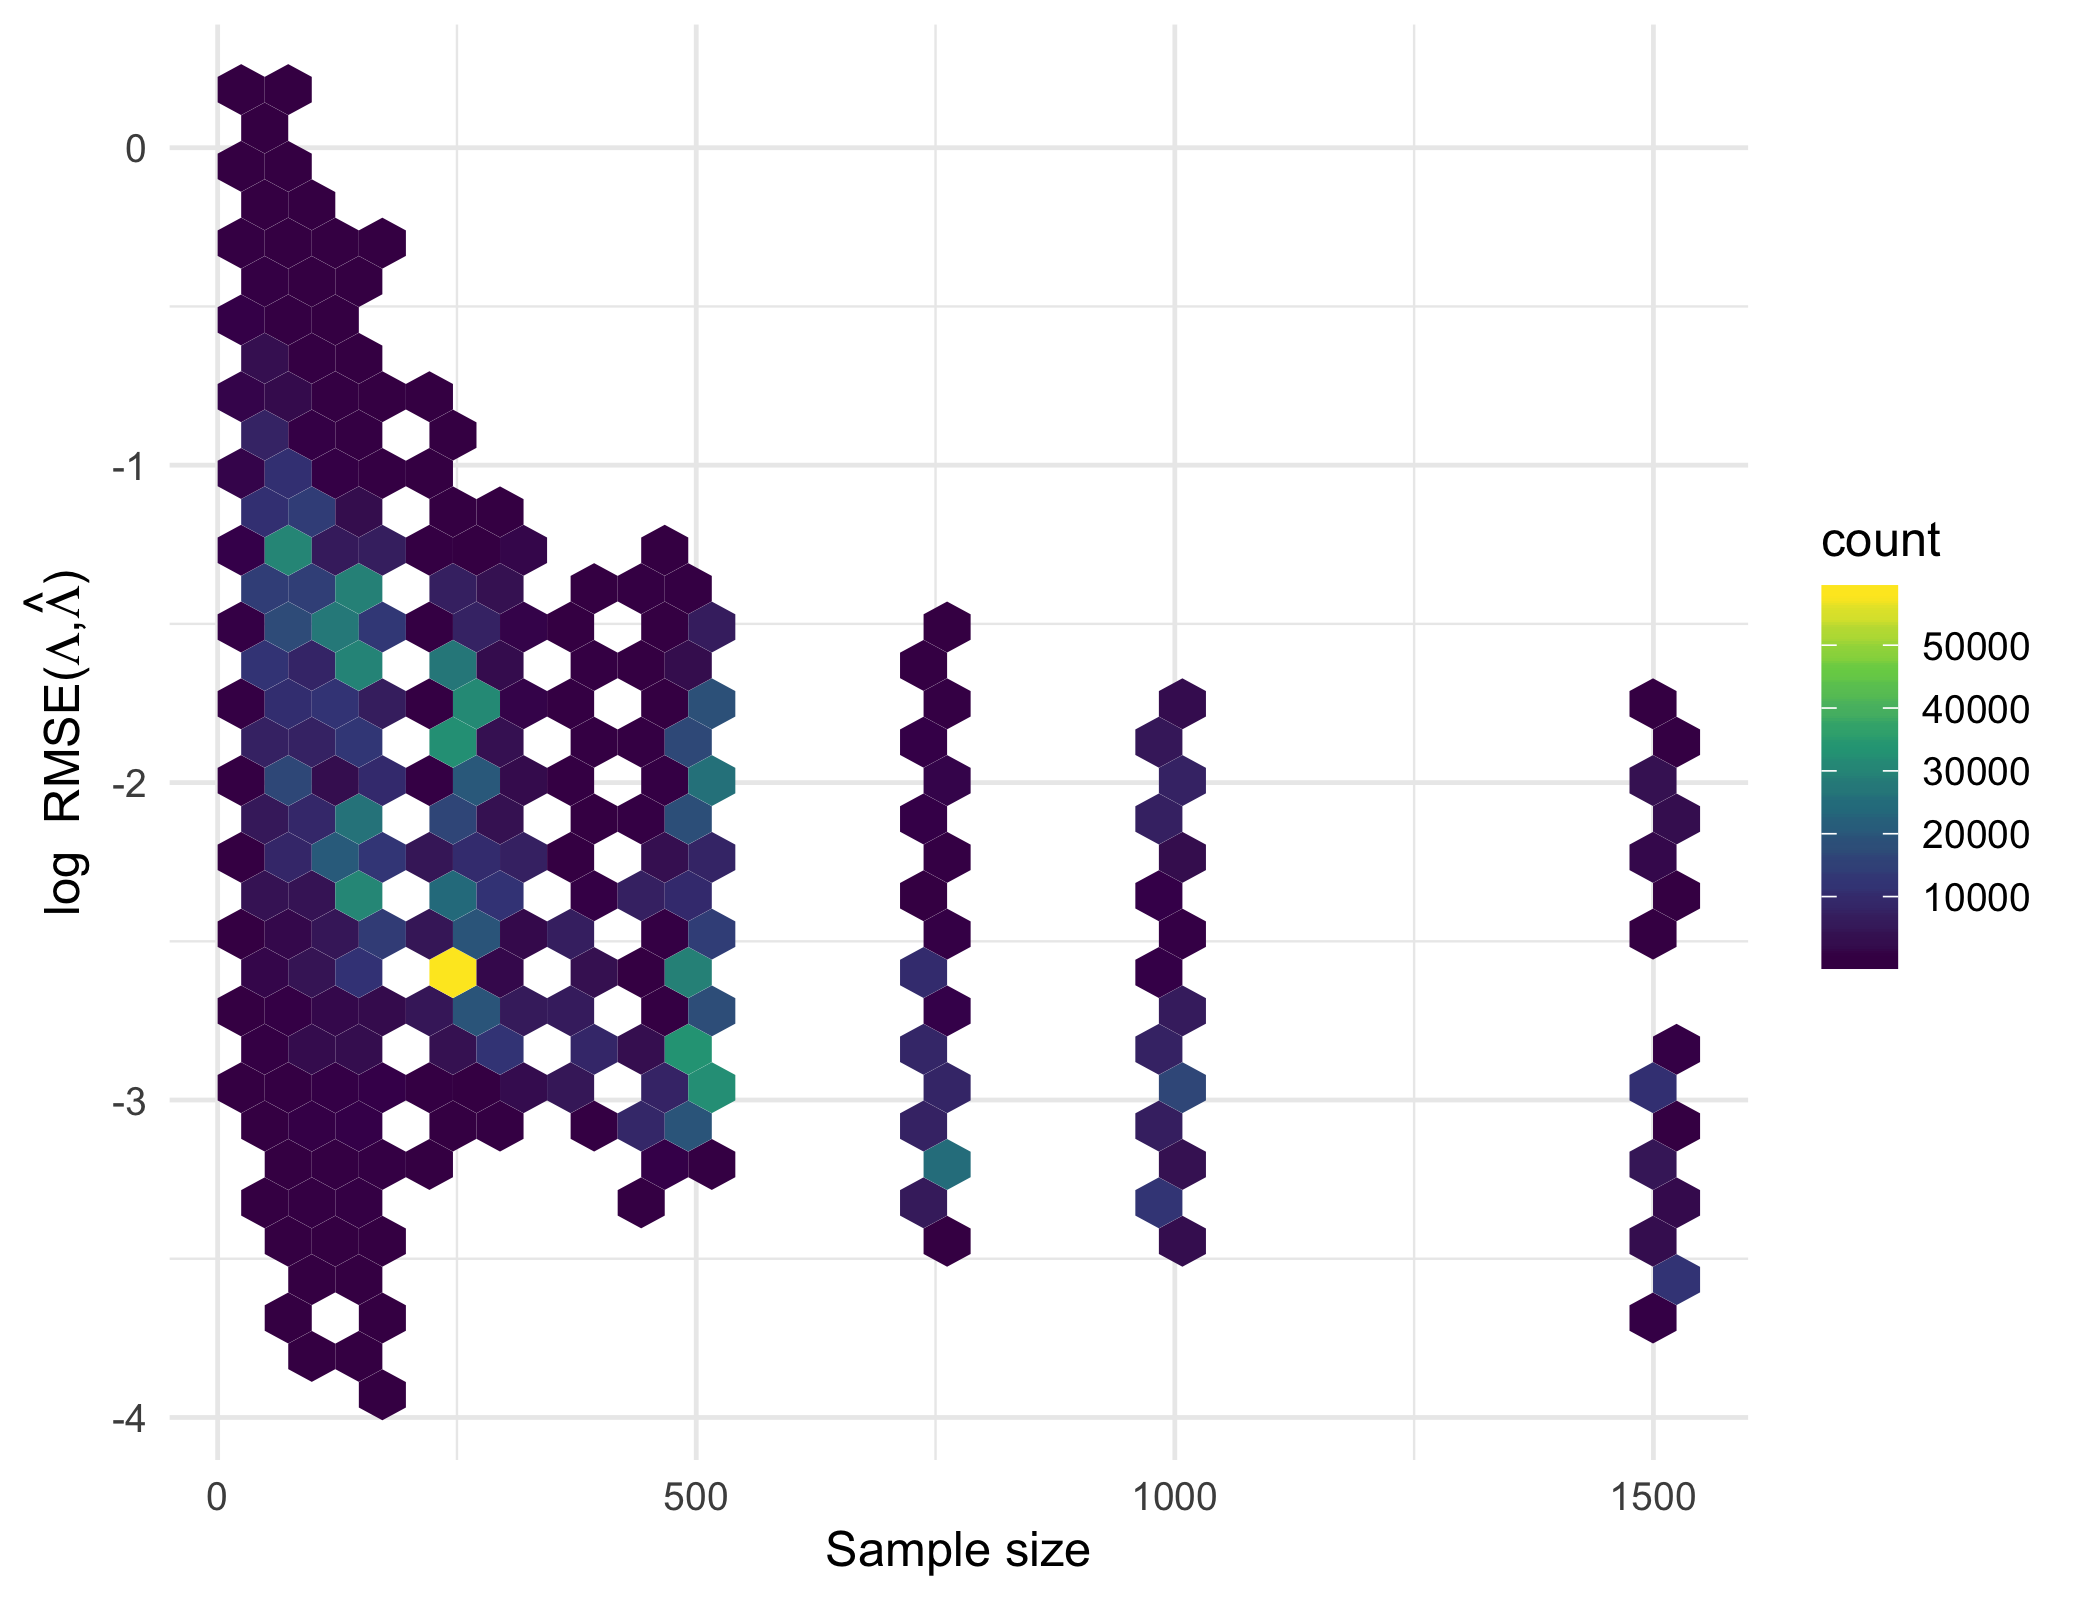
\includegraphics[width=6.5in]{/home/justin/Documents/masters_thesis/Text/figs/rmse_sample_size} 

}

\caption{Log root-mean-square error (RMSE) between the true and estimated factor loading matrices as a function of sample size.}\label{fig:RMSE-sample-size}
\end{figure}

\hypertarget{discussion}{%
\section{Discussion}\label{discussion}}

The current study examined how the application of three matrix smoothing algorithms (the Higham {[}2002{]}, Bentler-Yuan {[}2011{]}, and Knol-Berger {[}1991{]} algorithms) to indefinite tetrachoric correlation matrices affected both (a) the recovery of the model-implied population correlation matrix (\(\mathbf{R}_{\textrm{Pop}}\)), and (b) the recovery of the population item factor loadings in EFA (compared to leaving the indefinite correlation matrices unsmoothed). With respect to recovery of \(\mathbf{R}_{\textrm{Pop}}\), I found that that three variables were most related to \(\mathrm{D}_{\mathrm{s}}(\mathbf{R}_{\textrm{Sm}}, \mathbf{R}_{\textrm{Pop}})\): (a) the number of major factors in the data-generating model, (b) the number of subjects per item, and (c) the number of items per (major) factor. Increases in any of these variables were associated with improved population correlation matrix recovery. I also found that choice of smoothing method was somewhat related to population correlation matrix recovery. Specifically, the application of any of the three investigated matrix smoothing algorithms led to smoothed matrices were slightly closer to the population correlation matrix (\(\mathbf{R}_{\textrm{Pop}}\)) than the unsmoothed, indefinite tetrachoric correlation matrices. The results indicated that although the three smoothing algorithms led to very similar \(\mathrm{D}_{\mathrm{s}}(\mathbf{R}_{\textrm{Sm}}, \mathbf{R}_{\textrm{Pop}})\) values in most conditions, the Bentler-Yuan algorithm (2011) led to slightly lower \(\mathrm{D}_{\mathrm{s}}(\mathbf{R}_{\textrm{Sm}}, \mathbf{R}_{\textrm{Pop}})\) values in conditions with few subjects per item, few items per factor, and low factor loadings.

Concerning factor loading recovery, the simulation study results indicated that choice of smoothing algorithm---or, in fact, whether smoothing was applied at all---was not an important determinant of factor loading recovery when EFA was applied to smoothed or unsmoothed indefinite tetrachoric correlation matrices. Similar to the previous analyses, the Bentler-Yuan algorithm (2011) led to slightly better results (i.e., lower \(\textrm{RMSE}(\mathbf{F}, \hat{\mathbf{F}})\) values) than the alternative smoothing methods when factor loadings were low and there were few items per factor. Moreover, the Bentler-Yuan algorithm led to slightly better results when paired with maximum likelihood factor extraction (ML) compared to when the ordinary least squares (OLS) or principal axis (PA) extraction methods were used. However, the differences between the four smoothing methods (in terms of \(\textrm{RMSE}(\mathbf{F}, \hat{\mathbf{F}})\) values) were never large enough to be of practical importance. Although smoothing method choice was not found to be important for determining factor loading recovery, many of the other design variables were found to be important. In particular, \(\textrm{RMSE}(\mathbf{F}, \hat{\mathbf{F}})\) values were smallest for conditions with high factor loadings, many items per factor, and with little or no model approximation error. Moreover, the results indicated that the OLS and PA factor extraction methods led to highly similar results under all conditions. ML factor extraction method led to better results than OLS and PA in conditions with low factor loadings, few items per factor, and few subjects per item. The results also indicated that factor loading recovery for ML was less affected by model approximation error than were OLS or PA.

The results of this simulation study concerning both population correlation matrix recovery (\(\mathrm{D}_{\mathrm{s}}(\mathbf{R}_{\textrm{Sm}}, \mathbf{R}_{\textrm{Pop}})\)) and population factor loading recovery (\(\textrm{RMSE}(\mathbf{F}, \hat{\mathbf{F}})\)) can be put in the context of previous research. First, the current results provided additional evidence that the application of matrix smoothing algorithms to indefinite tetrachoric correlation matrices led to, at most, only a small effect on factor loading estimates in subsequent factor analyses. This result lends additional support to the conclusion of Knol and Berger (1991) that the effect of applying matrix smoothing to indefinite tetrachoric correlation matrices prior to conducting factor analysis was negligible.

To the extent that there were small differences among the smoothing methods in terms of \(\mathrm{D}_{\mathrm{s}}(\mathbf{R}_{\textrm{Sm}}, \mathbf{R}_{\textrm{Pop}})\) and \(\textrm{RMSE}(\mathbf{F}, \hat{\mathbf{F}})\), the Bentler-Yuan algorithm (2011) tended to lead to slightly better results than the alternative algorithms. Although I am not aware of any previous comparisons of relative smoothing algorithm performance in terms of population correlation matrix or factor loading recovery, Debelak and Tran (2013) and Debelak and Tran (2016) both found that the Bentler-Yuan algorithm led to somewhat better results than the Higham (2002) or Knol-Berger (1991) algorithms used with indefinite polychoric correlation matrices in the context of parallel analysis. These results, combined with the results from the present study, suggest that the Bentler-Yuan algorithm (2011) should be the default choice for smoothing indefinite tetrachoric or polychoric correlation matrices prior to conducting parallel analysis or factor analysis.

\hypertarget{limitations-and-future-directions}{%
\subsection{Limitations and Future Directions}\label{limitations-and-future-directions}}

As with any simulation study, the present simulation design was not able to cover the full range of realistic data scenarios. For instance, the simulation design included only orthogonal population factor models and did not allow for correlated factors. Moreover, the present study only included factor models with equal numbers of salient items per factor and fixed, uniform factor loadings. It might be the case that these loading matrices were overly-simplified and not representative of real data. Future research on this topic should investigate whether more complex factor loading and correlation structures affect the performance of matrix smoothing algorithms in terms of population correlation matrix recovery and factor loading recovery. Additionally, the present study only investigated the effects of matrix smoothing on indefinite tetrachoric correlation matrices. Further research should be done to investigate the effects of matrix smoothing on indefinite polychoric correlation matrices, as well as correlation matrices that are indefinite due to other causes such as indefinite correlation matrices calculated using pairwise deletion (Wothke, 1993) or composite correlation matrices used in meta-analysis (Furlow \& Beretvas, 2005). Little is known about whether the mechanism or \enquote{cause} of indefinite correlation matrices affects their structure, or how these potential differences might interact with the application of matrix smoothing algorithms.

Future research should also investigate ways to side-step the problem of indefinite tetrachoric correlation matrices. For instance, Choi, Kim, Chen, and Dannels (2011) found that polychoric correlation matrices estimated using expected a posteriori (EAP) rather than maximum-likelihood estimation led to estimates that were negatively biased but produced comparable (or smaller) RMSE values in terms of recovering the \enquote{true} correlations. It seems plausible that the slight shrinkage induced by using EAP as an estimation method would make indefinite tetrachoric or polychoric correlation matrices less common. Finally, full-information maximum likelihood (FIML; Bock \& Aitkin, 1981) can be used to estimate model parameters directly and doesn't require the estimation of a tetrachoric correlation matrix. Future research should investigate whether the use of FIML (which is computationally intensive, particularly with large models) offers any benefit in terms of parameter recovery when applied to data sets corresponding to indefinite tetrachoric correlation matrices.

\hypertarget{conclusion}{%
\subsection{Conclusion}\label{conclusion}}

Despite the lackluster improvement in factor loading recovery when factor analysis was conducted on smoothed rather than indefinite tetrachoric correlation matrices, the application of one of the three investigated matrix smoothing algorithms on indefinite tetrachoric correlation matrices is still recommended. None of the smoothing algorithms regularly led to worse results (in terms of factor loading recovery) compared to the conditions where the indefinite correlation matrix was left unsmoothed. Moreover, all of the smoothing algorithms investigated in this study are computationally inexpensive and are readily available as functions in R packages. For instance, the \emph{fungible} (Waller, 2019), \emph{sfsmisc} (Maechler, 2019), and \emph{Matrix} (Bates \& Maechler, 2019) packages all contain implementations of at least one of the three smoothing algorithms discussed in this article. In particular, the Bentler-Yuan algorithm (2011) often led to results that were at least as good (and sometimes slightly better) than the alternative smoothing algorithms and therefore seems a default choice of smoothing algorithm. Where the Bentler-Yuan algorithm is not available, the Knol-Berger algorithm (1991) is an alternative that is fast, easily implemented in most programming languages, does not have convergence issues, and generally led to results comparable to the Bentler-Yuan algorithm.

These recommendations come with a strong caveat. Namely, no matrix smoothing algorithm can reasonably be considered a remedy or solution for indefinite tetrachoric correlation matrices. Instead, researchers should consider indefinite tetrachoric correlation matrices to be symptoms of larger problems (e.g., small sample sizes, bad items, etc.) and be aware that practical solutions such as gathering more data or discarding bad items are likely to lead to better results than the application of matrix smoothing algorithms. In particular, indefinite tetrachoric correlation matrices are less likely to occur when sample sizes are large relative to the number of items (see Table 1 in Debelak \& Tran, 2013, p. 70), allowing researchers to avoid the question of how to properly deal with an indefinite tetrachoric correlation matrix entirely. If collecting more data is not possible, researchers should consider removing problematic items. In short, all three investigated smoothing algorithms are reasonable choices for dealing with indefinite tetrachoric correlation matrices prior to factor analysis and seem to offer a modest benefit (in terms of factor loading recovery) compared to leaving the indefinite tetrachoric correlation matrix unsmoothed. However, the application of these algorithms should be considered to be little more than a band-aid fix that does not address the underlying issues leading to indefinite tetrachoric correlation matrices nor to a marked improvement in factor loading recovery.

\newpage

\hypertarget{references}{%
\section{References}\label{references}}

\begingroup
\setlength{\parindent}{-0.5in}
\setlength{\leftskip}{0.5in}

\hypertarget{refs}{}
\leavevmode\hypertarget{ref-akaike1973}{}%
Akaike, H. (1973). \emph{Information theory and an extension of the maximum likelihood principle}. (B. N. Petrov \& F. Caski, Eds.) (pp. 267--281). Budapest: Akademiai Kiado.

\leavevmode\hypertarget{ref-R-papaja}{}%
Aust, F., \& Barth, M. (2018). \emph{papaja: Create APA manuscripts with R Markdown}. Retrieved from \url{https://github.com/crsh/papaja}

\leavevmode\hypertarget{ref-banerjee2014}{}%
Banerjee, S., \& Roy, A. (2014). \emph{Linear algebra and matrix analysis for statistics}. Chapman; Hall/CRC. \url{https://doi.org/10.1201/b17040}

\leavevmode\hypertarget{ref-R-questionr}{}%
Barnier, J., Briatte, F., \& Larmarange, J. (2018). \emph{Questionr: Functions to make surveys processing easier}. Retrieved from \url{https://CRAN.R-project.org/package=questionr}

\leavevmode\hypertarget{ref-R-Matrix}{}%
Bates, D., \& Maechler, M. (2019). \emph{Matrix: Sparse and dense matrix classes and methods}. Retrieved from \url{https://CRAN.R-project.org/package=Matrix}

\leavevmode\hypertarget{ref-R-lme4}{}%
Bates, D., Mächler, M., Bolker, B., \& Walker, S. (2015). Fitting linear mixed-effects models using lme4. \emph{Journal of Statistical Software}, \emph{67}(1), 1--48. \url{https://doi.org/10.18637/jss.v067.i01}

\leavevmode\hypertarget{ref-bentler1972}{}%
Bentler, P. (1972). A lower-bound method for the dimension-free measurement of internal consistency. \emph{Social Science Research}, \emph{1}(4), 343--357. \url{https://doi.org/10.1016/0049-089X(72)90082-8}

\leavevmode\hypertarget{ref-bentler2011}{}%
Bentler, P., \& Yuan, K.-H. (2011). Positive definiteness via off-diagonal scaling of a symmetric indefinite matrix. \emph{Psychometrika}, \emph{76}(1), 119--123. \url{https://doi.org/10.1007/s11336-010-9191-3}

\leavevmode\hypertarget{ref-birnbaum1968some}{}%
Birnbaum, A. L. (1968). Some latent trait models and their use in inferring an examinee's ability. \emph{Statistical Theories of Mental Test Scores}.

\leavevmode\hypertarget{ref-bock1981}{}%
Bock, R. D., \& Aitkin, M. (1981). Marginal maximum likelihood estimation of item parameters: Application of an em algorithm. \emph{Psychometrika}, \emph{46}(4), 443--459. \url{https://doi.org/10.1007/BF02293801}

\leavevmode\hypertarget{ref-bock1988}{}%
Bock, R. D., Gibbons, R., \& Muraki, E. (1988). Full-information item factor analysis. \emph{Applied Psychological Measurement}, \emph{12}(3), 261--280. \url{https://doi.org/10.1177/014662168801200305}

\leavevmode\hypertarget{ref-R-broom.mixed}{}%
Bolker, B., \& Robinson, D. (2019). \emph{Broom.mixed: Tidying methods for mixed models}. Retrieved from \url{https://CRAN.R-project.org/package=broom.mixed}

\leavevmode\hypertarget{ref-box1964}{}%
Box, G. E., \& Cox, D. R. (1964). An analysis of transformations. \emph{Journal of the Royal Statistical Society: Series B (Methodological)}, \emph{26}(2), 211--243. \url{https://doi.org/10.1111/j.2517-6161.1964.tb00553.x}

\leavevmode\hypertarget{ref-briggs2003}{}%
Briggs, N. E., \& MacCallum, R. C. (2003). Recovery of weak common factors by maximum likelihood and ordinary least squares estimation. \emph{Multivariate Behavioral Research}, \emph{38}(1), 25--56. \url{https://doi.org/10.1207/S15327906MBR3801_2}

\leavevmode\hypertarget{ref-brown1977mean}{}%
Brown, M. B., \& Benedetti, J. K. (1977). On the mean and variance of the tetrachoric correlation coefficient. \emph{Psychometrika}, \emph{42}(3), 347--355. \url{https://doi.org/10.1007/BF02293655}

\leavevmode\hypertarget{ref-browne1968comparison}{}%
Browne, M. W. (1968). A comparison of factor analytic techniques. \emph{Psychometrika}, \emph{33}(3), 267--334. \url{https://doi.org/10.1007/BF02289327}

\leavevmode\hypertarget{ref-butler1992}{}%
Butler, S. M., \& Louis, T. A. (1992). Random effects models with non-parametric priors. \emph{Statistics in Medicine}, \emph{11}(14-15), 1981--2000. \url{https://doi.org/10.1002/sim.4780111416}

\leavevmode\hypertarget{ref-carroll1957}{}%
Carroll, J. B. (1957). Biquartimin criterion for rotation to oblique simple structure in factor analysis. \emph{Science}, \emph{126}, 1114--1115. \url{https://doi.org/10.1126/science.126.3283.1114}

\leavevmode\hypertarget{ref-choi2011}{}%
Choi, J., Kim, S., Chen, J., \& Dannels, S. (2011). A comparison of maximum likelihood and Bayesian estimation for polychoric correlation using monte carlo simulation. \emph{Journal of Educational and Behavioral Statistics}, \emph{36}(4), 523--549. \url{https://doi.org/10.3102/1076998610381398}

\leavevmode\hypertarget{ref-comrey1962minimum}{}%
Comrey, A. L. (1962). The minimum residual method of factor analysis. \emph{Psychological Reports}, \emph{11}(1), 15--18. \url{https://doi.org/10.2466/pr0.1962.11.1.15}

\leavevmode\hypertarget{ref-CrockerAlgina}{}%
Crocker, L., \& Algina, J. (1986). \emph{Introduction to classical and modern test theory.} Orlando, FL: Wadsworth Publishing.

\leavevmode\hypertarget{ref-cudeck1991model}{}%
Cudeck, R., \& Henly, S. J. (1991). Model selection in covariance structures analysis and the ``problem'' of sample size: A clarification. \emph{Psychological Bulletin}, \emph{109}(3), 512. \url{https://doi.org/10.1037/0033-2909.109.3.512}

\leavevmode\hypertarget{ref-de2013theory}{}%
de Ayala, R. J. (2013). \emph{The theory and practice of item response theory}. Guilford Publications.

\leavevmode\hypertarget{ref-debelak2013}{}%
Debelak, R., \& Tran, U. S. (2013). Principal component analysis of smoothed tetrachoric correlation matrices as a measure of dimensionality. \emph{Educational and Psychological Measurement}, \emph{73}(1), 63--77. \url{https://doi.org/10.1177/0013164412457366}

\leavevmode\hypertarget{ref-debelak2016}{}%
Debelak, R., \& Tran, U. S. (2016). Comparing the effects of different smoothing algorithms on the assessment of dimensionality of ordered categorical items with parallel analysis. \emph{PLOS ONE}, \emph{11}(2), 1--18. \url{https://doi.org/10.1371/journal.pone.0148143}

\leavevmode\hypertarget{ref-devlin1975robust}{}%
Devlin, S. J., Gnanadesikan, R., \& Kettenring, J. R. (1975). Robust estimation and outlier detection with correlation coefficients. \emph{Biometrika}, \emph{62}(3), 531--545. \url{https://doi.org/10.1093/biomet/62.3.531}

\leavevmode\hypertarget{ref-dillon1987}{}%
Dillon, W. R., Kumar, A., \& Mulani, N. (1987). Offending estimates in covariance structure analysis: Comments on the causes of and solutions to Heywood cases. \emph{Psychological Bulletin}, \emph{101}(1), 126. \url{https://doi.org/10.1037/0033-2909.101.1.126}

\leavevmode\hypertarget{ref-divgi1979}{}%
Divgi, D. R. (1979). Calculation of the tetrachoric correlation coefficient. \emph{Psychometrika}, \emph{44}(2), 169--172. \url{https://doi.org/10.1007/BF02293968}

\leavevmode\hypertarget{ref-dong1985non}{}%
Dong, H.-K. (1985). Non-Gramian and singular matrices in maximum likelihood factor analysis. \emph{Applied Psychological Measurement}, \emph{9}(4), 363--366. \url{https://doi.org/10.1177/014662168500900404}

\leavevmode\hypertarget{ref-dwyer1939contribution}{}%
Dwyer, P. S. (1939). The contribution of an orthogonal multiple factor solution to multiple correlation. \emph{Psychometrika}, \emph{4}(2), 163--171. \url{https://doi.org/10.1007/BF02288494}

\leavevmode\hypertarget{ref-fabrigar1999evaluating}{}%
Fabrigar, L. R., Wegener, D. T., MacCallum, R. C., \& Strahan, E. J. (1999). Evaluating the use of exploratory factor analysis in psychological research. \emph{Psychological Methods}, \emph{4}(3), 272. \url{https://doi.org/10.1037/1082-989X.4.3.272}

\leavevmode\hypertarget{ref-R-car}{}%
Fox, J., \& Weisberg, S. (2019). \emph{An R companion to applied regression} (Third). Thousand Oaks CA: Sage. Retrieved from \url{https://socialsciences.mcmaster.ca/jfox/Books/Companion/}

\leavevmode\hypertarget{ref-furlow2005}{}%
Furlow, C. F., \& Beretvas, S. N. (2005). Meta-analytic methods of pooling correlation matrices for structural equation modeling under different patterns of missing data. \emph{Psychological Methods}, \emph{10}(2), 227. \url{https://doi.org/10.1037/1082-989X.10.2.227}

\leavevmode\hypertarget{ref-fushiki2009}{}%
Fushiki, T. (2009). Estimation of positive semidefinite correlation matrices by using convex quadratic semidefinite programming. \emph{Neural Computation}, \emph{21}(7), 2028--2048. \url{https://doi.org/10.1162/neco.2009.04-08-765}

\leavevmode\hypertarget{ref-R-viridis}{}%
Garnier, S. (2018). \emph{Viridis: Default color maps from 'matplotlib'}. Retrieved from \url{https://CRAN.R-project.org/package=viridis}

\leavevmode\hypertarget{ref-R-arm}{}%
Gelman, A., \& Su, Y.-S. (2018). \emph{Arm: Data analysis using regression and multilevel/hierarchical models}. Retrieved from \url{https://CRAN.R-project.org/package=arm}

\leavevmode\hypertarget{ref-hair2018}{}%
Hair, J. F., Black, W. C., Babin, B. J., \& Anderson, R. E. (2018). \emph{Multivariate data analysis}. Cengage.

\leavevmode\hypertarget{ref-hastie2009}{}%
Hastie, T., Tibshirani, R., \& Friedman, J. (2009). \emph{The elements of statistical learning: Data mining, inference, and prediction} (Second Edition). New York, NY: Springer New York.

\leavevmode\hypertarget{ref-R-purrr}{}%
Henry, L., \& Wickham, H. (2019). \emph{Purrr: Functional programming tools}. Retrieved from \url{https://CRAN.R-project.org/package=purrr}

\leavevmode\hypertarget{ref-higham2002}{}%
Higham, N. J. (2002). Computing the nearest correlation matrix---a problem from finance. \emph{IMA Journal of Numerical Analysis}, \emph{22}(3), 329--343. \url{https://doi.org/10.1093/imanum/22.3.329}

\leavevmode\hypertarget{ref-hong1999}{}%
Hong, S. (1999). Generating correlation matrices with model error for simulation studies in factor analysis: A combination of the Tucker-Koopman-Linn model and Wijsman's algorithm. \emph{Behavior Research Methods, Instruments, \& Computers}, \emph{31}(4), 727--730. \url{https://doi.org/10.3758/BF03200754}

\leavevmode\hypertarget{ref-horn1965}{}%
Horn, J. L. (1965). A rationale and test for the number of factors in factor analysis. \emph{Psychometrika}, \emph{30}(2), 179--185. \url{https://doi.org/10.1007/BF02289447}

\leavevmode\hypertarget{ref-jacqmin2007}{}%
Jacqmin-Gadda, H., Sibillot, S., Proust, C., Molina, J.-M., \& Thiébaut, R. (2007). Robustness of the linear mixed model to misspecified error distribution. \emph{Computational Statistics \& Data Analysis}, \emph{51}(10), 5142--5154. \url{https://doi.org/10.1016/j.csda.2006.05.021}

\leavevmode\hypertarget{ref-jamshidian1998}{}%
Jamshidian, M., \& Bentler, P. M. (1998). A quasi-Newton method for minimum trace factor analysis. \emph{Journal of Statistical Computation and Simulation}, \emph{62}(1-2), 73--89. \url{https://doi.org/10.1080/00949659808811925}

\leavevmode\hypertarget{ref-jennrich2002}{}%
Jennrich, R. I. (2002). A simple general method for oblique rotation. \emph{Psychometrika}, \emph{67}(1), 7--19. \url{https://doi.org/10.1007/BF02294706}

\leavevmode\hypertarget{ref-knol1991}{}%
Knol, D. L., \& Berger, M. P. (1991). Empirical comparison between factor analysis and multidimensional item response models. \emph{Multivariate Behavioral Research}, \emph{26}(3), 457--477. \url{https://doi.org/10.1207/s15327906mbr2603_5}

\leavevmode\hypertarget{ref-R-merTools}{}%
Knowles, J. E., \& Frederick, C. (2019). \emph{MerTools: Tools for analyzing mixed effect regression models}. Retrieved from \url{https://CRAN.R-project.org/package=merTools}

\leavevmode\hypertarget{ref-robustlmm}{}%
Koller, M. (2016). robustlmm: An R package for robust estimation of linear mixed-effects models. \emph{Journal of Statistical Software}, \emph{75}(6), 1--24. \url{https://doi.org/10.18637/jss.v075.i06}

\leavevmode\hypertarget{ref-kshirsagar1959bartlett}{}%
Kshirsagar, A. M. (1959). Bartlett decomposition and Wishart distribution. \emph{The Annals of Mathematical Statistics}, \emph{30}(1), 239--241. \url{https://doi.org/10.1214/aoms/1177706379}

\leavevmode\hypertarget{ref-R-texreg}{}%
Leifeld, P. (2013). texreg: Conversion of statistical model output in R to LaTeX and HTML tables. \emph{Journal of Statistical Software}, \emph{55}(8), 1--24. \url{https://doi.org/10.18637/jss.v055.i08}

\leavevmode\hypertarget{ref-li2010}{}%
Li, Q., Li, D., \& Qi, H. (2010). Newton's method for computing the nearest correlation matrix with a simple upper bound. \emph{Journal of Optimization Theory and Applications}, \emph{147}(3), 546--568. \url{https://doi.org/10.1007/s10957-010-9738-6}

\leavevmode\hypertarget{ref-lorenzoseva2020}{}%
Lorenzo-Seva, U., \& Ferrando, P. J. (2020). Not positive definite correlation matrices in exploratory item factor analysis: Causes, consequences and a proposed solution. \emph{Structural Equation Modeling: A Multidisciplinary Journal}, 1--10. \url{https://doi.org/10.1080/10705511.2020.1735393}

\leavevmode\hypertarget{ref-lurie1998}{}%
Lurie, P. M., \& Goldberg, M. S. (1998). An approximate method for sampling correlated random variables from partially-specified distributions. \emph{Management Science}, \emph{44}(2), 203--218. \url{https://doi.org/10.1287/mnsc.44.2.203}

\leavevmode\hypertarget{ref-maccallum1991representing}{}%
MacCallum, R. C., \& Tucker, L. R. (1991). Representing sources of error in the common-factor model: Implications for theory and practice. \emph{Psychological Bulletin}, \emph{109}(3), 502. \url{https://doi.org/10.1037/0033-2909.109.3.502}

\leavevmode\hypertarget{ref-maccallum2001}{}%
MacCallum, R. C., Widaman, K. F., Preacher, K. J., \& Hong, S. (2001). Sample size in factor analysis: The role of model error. \emph{Multivariate Behav. Res.}, \emph{36}(4), 611--637. \url{https://doi.org/10.1207/S15327906MBR3604_06}

\leavevmode\hypertarget{ref-R-sfsmisc}{}%
Maechler, M. (2019). \emph{Sfsmisc: Utilities from 'seminar fuer statistik' eth zurich}. Retrieved from \url{https://CRAN.R-project.org/package=sfsmisc}

\leavevmode\hypertarget{ref-magnus2019matrix}{}%
Magnus, J. R., \& Neudecker, H. (2019). \emph{Matrix differential calculus with applications in statistics and econometrics}. John Wiley \& Sons. \url{https://doi.org/10.1002/9781119541219}

\leavevmode\hypertarget{ref-R-wordcountaddin}{}%
Marwick, B. (2019). \emph{Wordcountaddin: Word counts and readability statistics in r markdown documents}. Retrieved from \url{https://github.com/benmarwick/wordcountaddin}

\leavevmode\hypertarget{ref-R-latex2exp}{}%
Meschiari, S. (2015). \emph{Latex2exp: Use latexexpressions in plots}. Retrieved from \url{https://CRAN.R-project.org/package=latex2exp}

\leavevmode\hypertarget{ref-R-koRpus}{}%
Michalke, M. (2018a). \emph{KoRpus: An r package for text analysis}. Retrieved from \url{https://reaktanz.de/?c=hacking\&s=koRpus}

\leavevmode\hypertarget{ref-R-sylly}{}%
Michalke, M. (2018b). \emph{Sylly: Hyphenation and syllable counting for text analysis}. Retrieved from \url{https://reaktanz.de/?c=hacking\&s=sylly}

\leavevmode\hypertarget{ref-R-koRpus.lang.en}{}%
Michalke, M. (2019). \emph{KoRpus.lang.en: Language support for 'koRpus' package: English}. Retrieved from \url{https://reaktanz.de/?c=hacking\&s=koRpus}

\leavevmode\hypertarget{ref-mulaik2009foundations}{}%
Mulaik, S. A. (2009). \emph{Foundations of factor analysis}. Chapman; Hall/CRC. \url{https://doi.org/10.1201/b15851}

\leavevmode\hypertarget{ref-R-here}{}%
Müller, K. (2017). \emph{Here: A simpler way to find your files}. Retrieved from \url{https://CRAN.R-project.org/package=here}

\leavevmode\hypertarget{ref-R-tibble}{}%
Müller, K., \& Wickham, H. (2019). \emph{Tibble: Simple data frames}. Retrieved from \url{https://CRAN.R-project.org/package=tibble}

\leavevmode\hypertarget{ref-olsson1979maximum}{}%
Olsson, U. (1979). Maximum likelihood estimation of the polychoric correlation coefficient. \emph{Psychometrika}, \emph{44}(4), 443--460. \url{https://doi.org/10.1007/BF02296207}

\leavevmode\hypertarget{ref-R-patchwork}{}%
Pedersen, T. L. (2019). \emph{Patchwork: The composer of plots}. Retrieved from \url{https://CRAN.R-project.org/package=patchwork}

\leavevmode\hypertarget{ref-qi2006}{}%
Qi, H., \& Sun, D. (2006). A quadratically convergent Newton method for computing the nearest correlation matrix. \emph{SIAM Journal on Matrix Analysis and Applications}, \emph{28}(2), 360--385. \url{https://doi.org/10.1137/050624509}

\leavevmode\hypertarget{ref-R-base}{}%
R Core Team. (2019). \emph{R: A language and environment for statistical computing}. Vienna, Austria: R Foundation for Statistical Computing. Retrieved from \url{https://www.R-project.org/}

\leavevmode\hypertarget{ref-roff1936some}{}%
Roff, M. (1936). Some properties of the communality in multiple factor theory. \emph{Psychometrika}, \emph{1}(2), 1--6. \url{https://doi.org/10.1007/BF02287999}

\leavevmode\hypertarget{ref-R-lattice}{}%
Sarkar, D. (2008). \emph{Lattice: Multivariate data visualization with R}. New York: Springer. \url{https://doi.org/10.1007/978-0-387-75969-2}

\leavevmode\hypertarget{ref-thurstone1947multiple}{}%
Thurstone, L. L. (1947). \emph{Multiple-factor analysis; a development and expansion of the vectors of mind} (pp. xix, 535). University of Chicago Press.

\leavevmode\hypertarget{ref-tucker1969}{}%
Tucker, L. R., Koopman, R. F., \& Linn, R. L. (1969). Evaluation of factor analytic research procedures by means of simulated correlation matrices. \emph{Psychometrika}, \emph{34}(4), 421--459. \url{https://doi.org/10.1007/BF02290601}

\leavevmode\hypertarget{ref-R-MASS}{}%
Venables, W. N., \& Ripley, B. D. (2002). \emph{Modern applied statistics with S} (Fourth). New York: Springer. \url{https://doi.org/10.1007/978-0-387-21706-2}

\leavevmode\hypertarget{ref-verbeke1997}{}%
Verbeke, G., \& Lesaffre, E. (1997). The effect of misspecifying the random-effects distribution in linear mixed models for longitudinal data. \emph{Computational Statistics \& Data Analysis}, \emph{23}(4), 541--556. \url{https://doi.org/10.1016/S0167-9473(96)00047-3}

\leavevmode\hypertarget{ref-R-fungible}{}%
Waller, N. G. (2019). \emph{Fungible: Psychometric functions from the Waller lab.}

\leavevmode\hypertarget{ref-R-ggplot2}{}%
Wickham, H. (2016). \emph{Ggplot2: Elegant graphics for data analysis}. Springer-Verlag New York. \url{https://doi.org/10.1007/978-3-319-24277-4}

\leavevmode\hypertarget{ref-R-forcats}{}%
Wickham, H. (2019a). \emph{Forcats: Tools for working with categorical variables (factors)}. Retrieved from \url{https://CRAN.R-project.org/package=forcats}

\leavevmode\hypertarget{ref-R-stringr}{}%
Wickham, H. (2019b). \emph{Stringr: Simple, consistent wrappers for common string operations}. Retrieved from \url{https://CRAN.R-project.org/package=stringr}

\leavevmode\hypertarget{ref-R-tidyverse}{}%
Wickham, H., Averick, M., Bryan, J., Chang, W., McGowan, L. D., François, R., \ldots{} Yutani, H. (2019). Welcome to the tidyverse. \emph{Journal of Open Source Software}, \emph{4}(43), 1686. \url{https://doi.org/10.21105/joss.01686}

\leavevmode\hypertarget{ref-R-dplyr}{}%
Wickham, H., François, R., Henry, L., \& Müller, K. (2019). \emph{Dplyr: A grammar of data manipulation}. Retrieved from \url{https://CRAN.R-project.org/package=dplyr}

\leavevmode\hypertarget{ref-R-tidyr}{}%
Wickham, H., \& Henry, L. (2019). \emph{Tidyr: Tidy messy data}. Retrieved from \url{https://CRAN.R-project.org/package=tidyr}

\leavevmode\hypertarget{ref-R-readr}{}%
Wickham, H., Hester, J., \& Francois, R. (2018). \emph{Readr: Read rectangular text data}. Retrieved from \url{https://CRAN.R-project.org/package=readr}

\leavevmode\hypertarget{ref-widaman1985iterative}{}%
Widaman, K. F., \& Herringer, L. G. (1985). Iterative least squares estimates of communality: Initial estimate need not affect stabilized value. \emph{Psychometrika}, \emph{50}(4), 469--477. \url{https://doi.org/10.1007/BF02296264}

\leavevmode\hypertarget{ref-wirth2007item}{}%
Wirth, R., \& Edwards, M. C. (2007). Item factor analysis: Current approaches and future directions. \emph{Psychological Methods}, \emph{12}(1), 58. \url{https://doi.org/10.1037/1082-989X.12.1.58}

\leavevmode\hypertarget{ref-wothke1993}{}%
Wothke, W. (1993). Testing structural equation models. In K. A. Bollen \& J. S. Long (Eds.), \emph{Testing structural equation models} (pp. 256--293). A Sage Focus Edition.

\leavevmode\hypertarget{ref-R-knitr}{}%
Xie, Y. (2015). \emph{Dynamic documents with R and knitr} (2nd ed.). Boca Raton, Florida: Chapman; Hall/CRC. \url{https://doi.org/10.1201/b15166}

\leavevmode\hypertarget{ref-zhang2001}{}%
Zhang, D., \& Davidian, M. (2001). Linear mixed models with flexible distributions of random effects for longitudinal data. \emph{Biometrics}, \emph{57}(3), 795--802. \url{https://doi.org/10.1111/j.0006-341X.2001.00795.x}

\endgroup


\clearpage
\renewcommand{\listfigurename}{Figure captions}

\clearpage
\renewcommand{\listtablename}{Table captions}


\clearpage
\makeatletter
\efloat@restorefloats
\makeatother


\begin{appendix}
\hypertarget{regression-diagnostics}{%
\section{Regression Diagnostics}\label{regression-diagnostics}}

\hypertarget{models-1a-and-1b-regression-models-predicting-log-textrmd_smathbfr_textrmsm-mathbfr_textrmpop}{%
\subsection{\texorpdfstring{Models 1A and 1B: Regression models
predicting
\(\log \textrm{D}_s(\mathbf{R}_{\textrm{Sm}}, \mathbf{R}_{\textrm{Pop}})\)}{Models 1A and 1B: Regression models predicting \textbackslash log \textbackslash textrm\{D\}\_s(\textbackslash mathbf\{R\}\_\{\textbackslash textrm\{Sm\}\}, \textbackslash mathbf\{R\}\_\{\textbackslash textrm\{Pop\}\})}}\label{models-1a-and-1b-regression-models-predicting-log-textrmd_smathbfr_textrmsm-mathbfr_textrmpop}}

Models 1A and 1B were a linear mixed-effects models predicting the (log)
scaled distance between the smoothed and model-implied population
correlation matrix and was fit using the R \emph{lme4} package (Version
1.1.23; Bates, Mächler, Bolker, \& Walker, 2015). Model 1A was a linear
model fit using all simulation variables and their interactions. In
Model 1B, second-degree polynomial terms were added for number of
factors, number of subjects per item, factor loading, and model error.
Diagnostic plots showing standardized residuals plotted against fitted
values for both models, quantile-quantile (QQ) plots of the residuals,
and QQ plots for the random intercept terms are shown in Figures
\ref{fig:residuals-vs-fitted-RpopRsm}, \ref{fig:qq-plot-RpopRsm}, and
\ref{fig:qq-plot-randInt-RpopRsm} respectively. These plots show that
some assumptions of the linear mixed-effects model seem to have been
violated for Models 1A and 1B, even after applying a log-transformation
to the response variable.

\begin{figure}

{\centering \includegraphics[width=7.54in]{/home/justin/Documents/masters_thesis/Text/figs/RpopRsm_resid_qq} 

}

\caption{Quantile-quantile plot of residuals for Models 1A and 1B.}\label{fig:qq-plot-RpopRsm}
\end{figure}

\begin{figure}

{\centering \includegraphics[width=7.54in]{/home/justin/Documents/masters_thesis/Text/figs/RpopRsm_ranef_qq} 

}

\caption{Quantile-quantile plot of random intercept terms for Models 1A and 1B.}\label{fig:qq-plot-randInt-RpopRsm}
\end{figure}

Figure \ref{fig:residuals-vs-fitted-RpopRsm} shows that the variance of
the residuals was not constant over the range of fitted values for both
the linear and polynomial models. In particular, for both models there
was little variation near the edges of the range of fitted values and a
large amount of variation near the center of the distribution of fitted
values. Therefore, the homoscedasticity assumption seemed to have been
violated. Moreover, Figure \ref{fig:qq-plot-RpopRsm} shows that the
assumption of normally-distributed errors was also likely violated. In
particular, Figure \ref{fig:qq-plot-RpopRsm} shows that the
distributions of residuals (for both models) had heavy tails and had a
slight positive skew (Model 1A: kurtosis = 16.25, skew = 0.60; Model 1B:
kurtosis = 18.61, skew = 0.23). Finally, Figure
\ref{fig:qq-plot-randInt-RpopRsm} shows that the random effects (random
intercepts) were not normally-distributed for either the linear or
polynomial model (Model 1A: kurtosis = 5.52, skew = 1.52; Model 1B:
kurtosis = 10.33, skew = 0.59). To address these violations of the model
assumptions, I first attempted to fit a robust mixed-effects model using
\texttt{rlmer()} function in the R \emph{robustlmm} package (Version
2.3; Koller, 2016). Unfortunately, the data set was too large for the
\texttt{rlmer()} function to handle. I also tried a more complex
transformation of the dependent variable (using a Box-Cox power
transformation; Box \& Cox, 1964), but it produced no discernible
benefit compared to a log transformation.

\begin{figure}

{\centering \includegraphics[width=7.54in]{/home/justin/Documents/masters_thesis/Text/figs/RpopRsm_resid_vs_fitted} 

}

\caption{Residuals plotted against fitted values for Models 1A and 1B.}\label{fig:residuals-vs-fitted-RpopRsm}
\end{figure}

The apparent violations of the assumptions of the mixed-effects model
were concerning. However, inference for the fixed effects in
mixed-effects models seems to be somewhat robust to these violations. In
particular, Jacqmin-Gadda, Sibillot, Proust, Molina, \& Thiébaut (2007)
showed that inference for fixed effects is robust for non-Gaussian and
heteroscedastic errors. Moreover, Jacqmin-Gadda et al.~(2007) cited
several studies indicating that inference for fixed effects is also
robust to non-Gaussian random effects (Butler \& Louis, 1992; Verbeke \&
Lesaffre, 1997; Zhang \& Davidian, 2001). Finally, the purpose of the
present analysis was to obtain estimates of the fixed effects of matrix
smoothing methods (and the interactions between smoothing methods and
the other design factors) on population correlation matrix recovery.
Neither \(p\)-values nor confidence intervals were of primary concern.
Therefore, the apparent violation of some model assumptions likely did
not affect the main results of this study.

\hypertarget{models-2a-and-2b-regression-models-predicting-log-textrmrmsemathbff-hatmathbff}{%
\subsection{\texorpdfstring{Models 2A and 2B: Regression models
predicting
\(\log \textrm{RMSE}(\mathbf{F}, \hat{\mathbf{F}})\)}{Models 2A and 2B: Regression models predicting \textbackslash log \textbackslash textrm\{RMSE\}(\textbackslash mathbf\{F\}, \textbackslash hat\{\textbackslash mathbf\{F\}\})}}\label{models-2a-and-2b-regression-models-predicting-log-textrmrmsemathbff-hatmathbff}}

Models 2A and 2B were mixed-effects models predicting
\(\log \textrm{RMSE}(\mathbf{F}, \hat{\mathbf{F}})\) and fit using the R
\emph{lme4} package (Bates, Mächler, Bolker, \& Walker, 2015). Model 2A
was a linear model fit using all simulation variables and their
interactions. In Model 2B, second-degree polynomial terms were added for
number of factors, number of subjects per item, factor loading, and
model error. As with Models 1A and 1B, diagnostic plots showing
standardized residuals plotted against fitted values for both models, QQ
plots for the residuals, and QQ plots for the random intercept terms are
shown in Figures \ref{fig:residuals-vs-fitted-RpopRsm},
\ref{fig:qq-plot-loading-recovery}, and
\ref{fig:qq-plot-randInt-loadings} respectively.

\begin{figure}

{\centering \includegraphics[width=7.54in]{/home/justin/Documents/masters_thesis/Text/figs/loading_resid_vs_fitted} 

}

\caption{Residuals plotted against fitted values for Models 2A and 2B.}\label{fig:residuals-vs-fitted-loading-recovery}
\end{figure}

\begin{figure}

{\centering \includegraphics[width=7.54in]{/home/justin/Documents/masters_thesis/Text/figs/loading_resid_qq} 

}

\caption{Quantile-quantile plot of residuals for Models 2A and 2B.}\label{fig:qq-plot-loading-recovery}
\end{figure}

\begin{figure}

{\centering \includegraphics[width=7.54in]{/home/justin/Documents/masters_thesis/Text/figs/loading_ranef_qq} 

}

\caption{Quantile-quantile plot of random intercept terms for Models 2A and 2B.}\label{fig:qq-plot-randInt-loadings}
\end{figure}

These plots indicate many of the same issues in Models 2A and 2B as were
seen for Models 1A and 1B. First, Figure
\ref{fig:residuals-vs-fitted-RpopRsm} shows clear evidence of
non-homogeneous conditional error variance for both the linear and
polynomial models. Specifically, the residual variance seemed generally
to be larger for larger fitted values. Second, Figure
\ref{fig:qq-plot-loading-recovery} shows that the distribution of
residuals for both models was non-normal and similar to the
distributions of the residuals from Model 1A and 1B (i.e.,
positively-skewed and having heavy tails). Finally, Figure
\ref{fig:qq-plot-randInt-loadings} shows that the estimated random
effects were likewise not normally-distributed. The distribution of
random intercepts was positively-skewed with heavy tails. Alternative
transformations of the dependent variable were tried but did not seem to
improve model fit compared to a log transformation. As with Model 1,
these violations of the model assumptions are somewhat concerning and
indicate that the estimated parameters---the estimated standard errors,
in particular---should be treated with some degree of skepticism.
However, the main results of the study are unlikely to have been
affected greatly by these violations of the model assumptions.
\end{appendix}

\clearpage
\makeatletter
\efloat@restorefloats
\makeatother


\begin{appendix}
\hypertarget{supplemental-tables-and-figures}{%
\section{Supplemental Tables and
Figures}\label{supplemental-tables-and-figures}}

\hypertarget{indefinite-matrix-frequency}{%
\subsection{Indefinite Matrix
Frequency}\label{indefinite-matrix-frequency}}

The percent of indefinite tetrachoric correlation matrices differed from
condition to condition. Table \ref{tab:percent-indefinite} reports the
percent of indefinite matrices for each of the 216 conditions of the
study design. One of the more obvious trends in this table is that
conditions with more (major) factors tended to produce more indefinite
tetrachoric correlation matrices. Based on the results reported by
Debelak and Tran (2013; 2016), who found that indefinite tetrachoric and
polychoric correlation matrices were much more common for data sets with
many items, this is likely due to the correlation of factor number with
total number of items. (See Lorenzo-Seva and Ferrando, 2020, for further
discussion of the relationship between the number of items and matrix
indefiniteness.) Moreover, the results in Table
\ref{tab:percent-indefinite} indicate that indefinite matrices were more
common for conditions with more items per factor, fewer subjects per
item, and higher factor loadings. All of these trends corroborate the
similar results by Debelak and Tran (2013; 2016) and their conclusions
about which variables most affected the frequency of indefinite
tetrachoric or polychoric correlation matrices.

\pagebreak

\begin{longtable}[t]{rrrrrrrr}
\caption{\label{tab:percent-indefinite}Percent of indefinite tetrachoric correlation
matrices by Number of Subjects Per Item (\(N/p\)), Number of Items per
Factor (\(p/m\)), Factor Loading, Model Error (\(\upsilon_\textrm{E}\)),
and Number of Factors.}\\
\toprule
\multicolumn{4}{c}{ } & \multicolumn{4}{c}{Factors} \\
\cmidrule(l{3pt}r{3pt}){5-8}
$N/p$ & $p/m$ & Loading & $\upsilon_{\textrm{E}}$ & 1 & 3 & 5 & 10\\
\midrule
5 & 5 & 0.3 & 0.0 & 10.5 & 96.6 & 100.0 & 100.0\\
5 & 5 & 0.3 & 0.1 & 10.6 & 97.3 & 100.0 & 100.0\\
5 & 5 & 0.3 & 0.3 & 13.5 & 99.3 & 100.0 & 100.0\\
5 & 5 & 0.5 & 0.0 & 15.6 & 98.9 & 100.0 & 100.0\\
5 & 5 & 0.5 & 0.1 & 14.4 & 99.0 & 100.0 & 100.0\\
5 & 5 & 0.5 & 0.3 & 15.6 & 100.0 & 100.0 & 100.0\\
5 & 5 & 0.8 & 0.0 & 13.5 & 100.0 & 100.0 & 100.0\\
5 & 5 & 0.8 & 0.1 & 13.4 & 100.0 & 100.0 & 100.0\\
5 & 5 & 0.8 & 0.3 & 13.9 & 100.0 & 100.0 & 100.0\\
5 & 10 & 0.3 & 0.0 & 78.0 & 100.0 & 100.0 & 100.0\\
5 & 10 & 0.3 & 0.1 & 79.1 & 100.0 & 100.0 & 100.0\\
5 & 10 & 0.3 & 0.3 & 85.5 & 100.0 & 100.0 & 100.0\\
5 & 10 & 0.5 & 0.0 & 88.1 & 100.0 & 100.0 & 100.0\\
5 & 10 & 0.5 & 0.1 & 89.3 & 100.0 & 100.0 & 100.0\\
5 & 10 & 0.5 & 0.3 & 94.1 & 100.0 & 100.0 & 100.0\\
5 & 10 & 0.8 & 0.0 & 98.9 & 100.0 & 100.0 & 100.0\\
5 & 10 & 0.8 & 0.1 & 99.3 & 100.0 & 100.0 & 100.0\\
5 & 10 & 0.8 & 0.3 & 99.6 & 100.0 & 100.0 & 100.0\\
10 & 5 & 0.3 & 0.0 & 2.5 & 7.9 & 9.4 & 5.8\\
10 & 5 & 0.3 & 0.1 & 2.0 & 10.5 & 12.3 & 18.1\\
10 & 5 & 0.3 & 0.3 & 3.3 & 26.8 & 54.6 & 93.1\\
10 & 5 & 0.5 & 0.0 & 3.4 & 21.3 & 29.0 & 49.1\\
10 & 5 & 0.5 & 0.1 & 3.5 & 26.0 & 38.1 & 70.8\\
10 & 5 & 0.5 & 0.3 & 4.4 & 48.8 & 82.5 & 99.7\\
10 & 5 & 0.8 & 0.0 & 13.1 & 98.4 & 100.0 & 100.0\\
10 & 5 & 0.8 & 0.1 & 11.4 & 98.2 & 100.0 & 100.0\\
10 & 5 & 0.8 & 0.3 & 12.5 & 99.3 & 100.0 & 100.0\\
10 & 10 & 0.3 & 0.0 & 8.7 & 8.0 & 7.9 & 5.1\\
10 & 10 & 0.3 & 0.1 & 11.0 & 14.0 & 19.5 & 38.2\\
10 & 10 & 0.3 & 0.3 & 21.2 & 70.2 & 94.4 & 100.0\\
10 & 10 & 0.5 & 0.0 & 23.8 & 39.5 & 63.3 & 94.8\\
10 & 10 & 0.5 & 0.1 & 24.2 & 56.3 & 83.7 & 99.9\\
10 & 10 & 0.5 & 0.3 & 39.8 & 94.4 & 100.0 & 100.0\\
10 & 10 & 0.8 & 0.0 & 84.2 & 100.0 & 100.0 & 100.0\\
10 & 10 & 0.8 & 0.1 & 83.3 & 100.0 & 100.0 & 100.0\\
10 & 10 & 0.8 & 0.3 & 89.9 & 100.0 & 100.0 & 100.0\\
15 & 5 & 0.3 & 0.0 & 0.4 & 0.0 & 0.0 & 0.0\\
15 & 5 & 0.3 & 0.1 & 0.2 & 0.1 & 0.0 & 0.0\\
15 & 5 & 0.3 & 0.3 & 0.8 & 1.4 & 1.2 & 0.9\\
15 & 5 & 0.5 & 0.0 & 0.8 & 0.8 & 0.0 & 0.0\\
15 & 5 & 0.5 & 0.1 & 0.5 & 1.1 & 0.7 & 0.2\\
15 & 5 & 0.5 & 0.3 & 1.0 & 4.9 & 7.9 & 18.7\\
15 & 5 & 0.8 & 0.0 & 9.4 & 65.9 & 87.4 & 100.0\\
15 & 5 & 0.8 & 0.1 & 9.3 & 69.1 & 92.1 & 100.0\\
15 & 5 & 0.8 & 0.3 & 9.3 & 85.4 & 99.2 & 100.0\\
15 & 10 & 0.3 & 0.0 & 0.3 & 0.0 & 0.0 & 0.0\\
15 & 10 & 0.3 & 0.1 & 0.5 & 0.0 & 0.0 & 0.0\\
15 & 10 & 0.3 & 0.3 & 3.7 & 2.2 & 1.1 & 2.0\\
15 & 10 & 0.5 & 0.0 & 2.8 & 0.3 & 0.0 & 0.0\\
15 & 10 & 0.5 & 0.1 & 3.6 & 0.5 & 0.0 & 0.1\\
15 & 10 & 0.5 & 0.3 & 7.1 & 14.5 & 29.8 & 78.0\\
15 & 10 & 0.8 & 0.0 & 51.0 & 96.4 & 100.0 & 100.0\\
15 & 10 & 0.8 & 0.1 & 51.8 & 99.2 & 100.0 & 100.0\\
15 & 10 & 0.8 & 0.3 & 65.9 & 100.0 & 100.0 & 100.0\\
\bottomrule
\end{longtable}






\pagebreak

\hypertarget{observed-textrmd_textrmsmathbfr_textrmsm-mathbfr_textrmpop-values}{%
\subsection{\texorpdfstring{Observed
\(\textrm{D}_{\textrm{s}}(\mathbf{R}_{\textrm{Sm}}, \mathbf{R}_{\textrm{Pop}})\)
Values}{Observed \textbackslash textrm\{D\}\_\{\textbackslash textrm\{s\}\}(\textbackslash mathbf\{R\}\_\{\textbackslash textrm\{Sm\}\}, \textbackslash mathbf\{R\}\_\{\textbackslash textrm\{Pop\}\}) Values}}\label{observed-textrmd_textrmsmathbfr_textrmsm-mathbfr_textrmpop-values}}

In addition to the estimated marginal means shown in the main text, the
following figures (Figures
\ref{fig:ds-one-factor}--\ref{fig:ds-ten-factor}) show box-plots of
\(\Ds\) for each condition in the simulation design. These box-plots
match well with the estimated marginal means shown in the main text.
However, notice that some conditions in these figures are missing
box-plots (e.g., three factors, 15 subjects per item, 10 items per
factor, \(\upsilon_\textrm{E} = 0\), and Loading = 0.3) because no
indefinite tetrachoric correlation matrices were produced for those
conditions.

\begin{figure}

{\centering \includegraphics[width=\textwidth]{/home/justin/Documents/masters_thesis/Text/figs/ds_boxplot_01_factor} 

}

\caption{$\textrm{D}_{\textrm{s}}(\mathbf{R}_{\textrm{Sm}}, \mathbf{R}_{\textrm{Pop}})$ values for one-factor models. APA = Higham (2002); BY = Bentler-Yuan (2011); KB = Knol-Berger (1991); None = no smoothing; $\upsilon_{\textrm{E}}$ = Proportion of uniqueness variance redistributed to the minor common factors representing model approximation error.}\label{fig:ds-one-factor}
\end{figure}

\begin{figure}

{\centering \includegraphics[width=\textwidth]{/home/justin/Documents/masters_thesis/Text/figs/ds_boxplot_03_factor} 

}

\caption{$\textrm{D}_{\textrm{s}}(\mathbf{R}_{\textrm{Sm}}, \mathbf{R}_{\textrm{Pop}})$ values for three-factor models. APA = Higham (2002); BY = Bentler-Yuan (2011); KB = Knol-Berger (1991); None = no smoothing; $\upsilon_{\textrm{E}}$ = Proportion of uniqueness variance redistributed to the minor common factors representing model approximation error.}\label{fig:ds-three-factor}
\end{figure}

\begin{figure}

{\centering \includegraphics[width=\textwidth]{/home/justin/Documents/masters_thesis/Text/figs/ds_boxplot_05_factor} 

}

\caption{$\textrm{D}_{\textrm{s}}(\mathbf{R}_{\textrm{Sm}}, \mathbf{R}_{\textrm{Pop}})$ values for five-factor models. APA = Higham (2002); BY = Bentler-Yuan (2011); KB = Knol-Berger (1991); None = no smoothing; $\upsilon_{\textrm{E}}$ = Proportion of uniqueness variance redistributed to the minor common factors representing model approximation error.}\label{fig:ds-five-factor}
\end{figure}

\begin{figure}

{\centering \includegraphics[width=\textwidth]{/home/justin/Documents/masters_thesis/Text/figs/ds_boxplot_10_factor} 

}

\caption{$\textrm{D}_{\textrm{s}}(\mathbf{R}_{\textrm{Sm}}, \mathbf{R}_{\textrm{Pop}})$ values for ten-factor models. APA = Higham (2002); BY = Bentler-Yuan (2011); KB = Knol-Berger (1991); None = no smoothing; $\upsilon_{\textrm{E}}$ = Proportion of uniqueness variance redistributed to the minor common factors representing model approximation error.}\label{fig:ds-ten-factor}
\end{figure}

\pagebreak

\hypertarget{observed-textrmrmsemathbff-hatmathbff-values}{%
\subsection{\texorpdfstring{Observed
\(\textrm{RMSE}(\mathbf{F}, \hat{\mathbf{F}})\)
Values}{Observed \textbackslash textrm\{RMSE\}(\textbackslash mathbf\{F\}, \textbackslash hat\{\textbackslash mathbf\{F\}\}) Values}}\label{observed-textrmrmsemathbff-hatmathbff-values}}

Figures \ref{fig:rmse-one-factor}--\ref{fig:rmse-ten-factor} in this
section show box-plots of
\(\textrm{RMSE}(\mathbf{F}, \hat{\mathbf{F}})\) for each condition in
the study design. Similar to the figures in the previous section, these
box-plots for the most part agree well with the estimated marginal means
presented in the main text, but are missing data for conditions with no
indefinite tetrachoric correlation matrices.

\begin{figure}

{\centering \includegraphics[width=6.74in]{/home/justin/Documents/masters_thesis/Text/figs/rmse_boxplot_01_factor} 

}

\caption{$\textrm{RMSE}(\mathbf{F}, \hat{\mathbf{F}})$ values for one-factor models. APA = Higham (2002); BY = Bentler-Yuan (2011); KB = Knol-Berger (1991); None = no smoothing; OLS = Ordinary least squares; ML = Maximum likelihood; PA = Principal axis; $\upsilon_{\textrm{E}}$ = Proportion of uniqueness variance redistributed to the minor common factors representing model approximation error.}\label{fig:rmse-one-factor}
\end{figure}

\begin{figure}

{\centering \includegraphics[width=6.74in]{/home/justin/Documents/masters_thesis/Text/figs/rmse_boxplot_03_factor} 

}

\caption{$\textrm{RMSE}(\mathbf{F}, \hat{\mathbf{F}})$ values for three-factor models. APA = Higham (2002); BY = Bentler-Yuan (2011); KB = Knol-Berger (1991); None = no smoothing; OLS = Ordinary least squares; ML = Maximum likelihood; PA = Principal axis; $\upsilon_{\textrm{E}}$ = Proportion of uniqueness variance redistributed to the minor common factors representing model approximation error.}\label{fig:rmse-three-factor}
\end{figure}

\begin{figure}

{\centering \includegraphics[width=6.74in]{/home/justin/Documents/masters_thesis/Text/figs/rmse_boxplot_05_factor} 

}

\caption{$\textrm{RMSE}(\mathbf{F}, \hat{\mathbf{F}})$ values for five-factor models. APA = Higham (2002); BY = Bentler-Yuan (2011); KB = Knol-Berger (1991); None = no smoothing; OLS = Ordinary least squares; ML = Maximum likelihood; PA = Principal axis; $\upsilon_{\textrm{E}}$ = Proportion of uniqueness variance redistributed to the minor common factors representing model approximation error.}\label{fig:rmse-five-factor}
\end{figure}

\begin{figure}

{\centering \includegraphics[width=6.74in]{/home/justin/Documents/masters_thesis/Text/figs/rmse_boxplot_10_factor} 

}

\caption{$\textrm{RMSE}(\mathbf{F}, \hat{\mathbf{F}})$ values for ten-factor models. APA = Higham (2002); BY = Bentler-Yuan (2011); KB = Knol-Berger (1991); None = no smoothing; OLS = Ordinary least squares; ML = Maximum likelihood; PA = Principal axis; $\upsilon_{\textrm{E}}$ = Proportion of uniqueness variance redistributed to the minor common factors representing model approximation error.}\label{fig:rmse-ten-factor}
\end{figure}
\end{appendix}

\end{document}
